\documentclass[11pt]{article}
\usepackage[margin=1in]{geometry}
\usepackage[T1]{fontenc}
\usepackage{amsmath,amssymb,amsthm,booktabs,graphicx,natbib,float,placeins,hyperref}
\hypersetup{colorlinks=true,citecolor=blue,urlcolor=blue,linkcolor=blue}
\newtheorem{proposition}{Proposition}
\title{Return forecasts and execution timing:\\A matched-endpoint study of cryptocurrency orders}
\author{Lai Jien Weng\\Monash University\\\texttt{lai.jienweng@monash.edu}}
\date{19 September 2026}
\begin{document}
\maketitle
\begin{abstract}
Forecasts used to schedule a required trade should be evaluated against the timing decision they support. Terminal-return accuracy alone leaves expected price differences across execution opportunities unspecified. We develop a transparent matched-endpoint diagnostic within a fixed-volume quadratic execution model and separate the resulting timing payoff from the cost of changing the schedule. Four forecast profiles share exactly the same terminal prediction but induce different schedules and objective outcomes. A retrospective Bitcoin--Ether study uses 699,840 one-minute observations and 17,664 hypothetical order episodes across six rolling evaluation months. Under the primary assumed cost specification, the learned profile produces an average gross timing benefit of 0.00370 basis points, below its 0.00805 basis-point scheduling cost, yielding a negative net gain. The negative average is concentrated in April. Historical attenuation changes this trade-off but does not establish reliable improvement; a lower-percentile policy selects the baseline throughout. The contribution is an operational comparison of forecast targets and decision consequences, supported by complete window-level results and reproducible diagnostics. The elementary execution principle is established in prior work, and the replay does not identify actual fills, market impact or commercially attainable savings.
\end{abstract}
\noindent\textbf{Keywords:} optimal execution; forecast evaluation; transaction costs; decision-focused prediction; Bitcoin; Ether.

\section{Introduction}\label{sec:intro}
A trader who has already committed to sell a fixed quantity faces a different problem from an investor deciding whether to hold an asset. The execution trader allocates the required quantity across available times. Predicting the final price can help with that task if it also reveals how prices are expected to evolve before completion. By itself, however, an accurate endpoint forecast does not specify whether the favourable trading opportunity occurs early, late or uniformly across the execution horizon. The distinction matters whenever a prediction system is evaluated using a statistical target that contains less information than the decision requires.

Optimal-execution research has long recognised the relevance of predictive information. Trading controls can respond to expected order flow, persistent signals and price changes over the remaining horizon \citep{cartea2016,lehalle2019,forde2022,abijaber2025}. A separate literature on decision-focused prediction shows why low forecast error need not imply a low downstream decision loss \citep{elmachtoub2022,mandi2024}. These are established motivations, rather than gaps discovered by this study. The more specific problem addressed here is how to make the omitted timing information visible in a small, reproducible evaluation while keeping terminal forecasts exactly comparable.

We approach that problem through a matched-endpoint construction. Starting from a learned vector of expected execution-slot prices, we form three additional profiles with the same final coordinate. A parallel profile assigns the endpoint value to every slot; a ramp imposes a linear path to that endpoint; and a mirror reverses the intermediate contrasts around the same endpoint. Consequently, all profiles receive identical terminal-return errors and directional-hit indicators on every observation. They can nevertheless induce different feasible schedules because their relative expected prices differ. The profiles are controlled diagnostic constructions, not a set of equally plausible trained forecasting competitors.

Matching endpoints identifies what an endpoint metric cannot distinguish, but does not determine whether acting on the learned profile is worthwhile. For that second question, we decompose the realised gain from a schedule change into a timing-price payoff, a first-order baseline-cost penalty and a quadratic deviation cost. The decomposition gives an explicit economic condition: full exposure is beneficial only when the timing payoff exceeds both cost terms. Positive gross alignment with realised prices is insufficient. This framework also separates a monetary execution charge from an inventory preference, so an improvement in the combined objective is not automatically a cash saving.

The empirical illustration uses public one-minute Binance observations for Bitcoin and Ether from January through August 2026. Six rolling windows per asset allocate one month to forecast estimation, the next to exposure calibration and the third to evaluation. The final evaluation sample contains 17,664 hypothetical order episodes over 184 calendar dates. The signal is a simple imbalance measure from five completed bars, and the schedule uses fifteen subsequent minute-open proxies. The deliberately limited forecasting model makes the comparison inspectable; its simplicity is not evidence that it is the best available cryptocurrency predictor.

Under the primary assumed impact and inventory parameters, the learned schedule earns an average gross timing payoff of 0.00370 basis points but incurs a curvature cost of 0.00805 basis points. Its net objective gain is therefore negative. A half-exposure schedule reduces both benefit and cost, while a historical plug-in coefficient selects positive exposure in six of twelve asset--month windows. The more conservative lower-percentile coefficient selects zero throughout. These outcomes support a reporting lesson about the cost of acting on a forecast; they do not establish superiority of a new trading rule. In particular, a positive realised timing payoff is an ex-post sample quantity, not proof of stable exploitable predictive information.

The study contributes an operational diagnostic, a worked benefit--cost accounting and a transparent multi-window illustration. Its main value is to make the evaluation target explicit: a required-order timing decision depends on temporal price contrasts and the costs induced by the chosen response. The mathematics does not constitute a new optimal-execution principle, and the crypto application itself has direct precedents \citep{bundi2024,schnaubelt2022}. The evidence is also retrospective: the expanded design followed an initial inspected Bitcoin window. Complete results, including adverse and inconclusive comparisons, are therefore reported as exploratory rather than presented as independent confirmation.

The rest of the paper follows the decision from context to evidence. Section~\ref{sec:literature} positions the diagnostic within predictive execution, decision-focused learning and crypto microstructure. Section~\ref{sec:methods} develops the fixed-volume accounting and the chronological replay. Section~\ref{sec:results} presents the matched-profile outcomes, variation across windows, exposure policies and cost sensitivity, followed by their economic interpretation. Section~\ref{sec:conclusion} states what the evidence establishes and what remains to be tested.

\section{Literature review}
\label{sec:literature}
\subsection{Predictive information and the timing of execution}
Optimal execution studies how to complete an order while balancing the consequences of trading quickly against those of carrying inventory. The impact--risk formulation of \citet{almgren2001} supplies a foundational benchmark. Once prices contain predictive information, the schedule also depends on when favourable prices are expected to occur. \citet{cartea2016} incorporate expected future net order flow, while \citet{bechler2015} study execution with dynamic order-flow imbalance. \citet{cartea2018} connect order-book signals to trading decisions. These studies motivate using an imbalance predictor, but do not establish that the coarser taker-volume measure available in minute bars contains the same information as an observed order book.

The relevant forecasting object is generally a temporal profile. \citet{lehalle2019} incorporate signals into execution and derive deterministic schedules conditional on initial information within part of their analysis. \citet{neuman2022} instead address signal-adaptive trading with temporary and transient impact. Learning latent alpha states provides another route for incorporating information into trading controls \citep{casgrain2019}. In the related portfolio-choice setting, \citet{garleanu2013} show why transaction costs and the persistence of return predictors affect dynamic adjustment. These formulations differ in information structure and feasible actions, so they should not be treated as interchangeable benchmarks for a schedule fixed at the start of an episode.

Two contributions are particularly close to the distinction developed here. \citet{forde2022} express predictive execution through expected remaining price changes in a Gaussian-signal model with power-law resilience. \citet{abijaber2025} use conditional price contrasts in a more general propagator framework. Their formulations already contain the economic reason that fixed-volume execution depends on relative prices across trading times. Recent work by \citet{bank2026} further develops execution and speculation with trade signals. Consequently, neither using forecasts in execution nor cancelling a common price-level component constitutes a new execution principle. Our narrower contribution is an observable diagnostic: holding the terminal forecast exactly fixed while changing the intrahorizon profile separates information captured by terminal prediction scores from information that can alter a schedule.

\subsection{Decision loss, calibration and model uncertainty}
The distinction between prediction quality and decision quality extends well beyond execution. \citet{elmachtoub2022} formulate learning around the loss induced by downstream optimization. \citet{liu2021} establish risk and calibration results for a related predict-then-optimize method under stated assumptions. The review and benchmark of \citet{mandi2024} place these approaches within decision-focused learning, while \citet{gupta2024} develop directional-gradient methods. Dependence in the training observations creates additional theoretical issues, as the preprint of \citet{liudependent2024} illustrates. Our analysis shares the motivation of evaluating forecasts through decisions, but does not train a new decision-focused predictor or establish comparable generalization bounds. Ordinary least squares is retained so that the decision diagnostic can be examined without attributing results to a complex forecasting architecture.

Economic forecast evaluation also appears in applied financial research. \citet{maciel2025}, for example, evaluates equity risk-premium forecasts through a portfolio allocation strategy. That application concerns investment exposure rather than the timing of a committed order. The distinction matters: an investor can change how much risk to hold, whereas every feasible schedule here must complete the same sale. A forecast of the final price may inform exposure choice while failing to distinguish competing execution profiles. The matched-endpoint comparison makes this restriction explicit, and the quadratic decomposition identifies both the gross price-alignment benefit and the extra scheduling cost.

Attenuating uncertain signals is likewise an established concern. \citet{kan2007} study portfolio choice under parameter uncertainty. \citet{cartea2017} address model uncertainty in algorithmic trading, and the liquidation working paper of \citet{cartea_liquidation2017} focuses on ambiguity aversion. \citet{horst2022} examine liquidation under factor uncertainty, while \citet{demarch2018} study signal-based trading with uncertainty and threshold behaviour. These approaches motivate caution about an estimated signal, but their objectives and uncertainty sets differ from a coefficient fitted on a preceding calibration month. We therefore interpret our coefficient as an empirical schedule weight, not as an ambiguity-robust optimum.

Uncertainty about execution costs is distinct from uncertainty about returns. \citet{fouque2022} jointly consider signals and stochastic price impact. The preprint of \citet{hey2023} examines the cost of misspecifying impact, and \citet{neumanoffline2023} develop an offline-learning approach to propagator models. \citet{macri2024} study reinforcement learning when liquidity varies over time. This strand limits what can be inferred from the present exercise: changing an assumed impact parameter is a sensitivity analysis, not an estimate of the impact that a real order would generate. A transparent small model helps locate the source of a replay result, but cannot substitute for measurements of depth, fills or endogenous price responses.

\subsection{Uncertainty gates and dependence-aware evaluation}
A particularly relevant recent comparator is \citet{irshad2026}, whose uncertainty-aware execution framework uses a conformal-prediction gate and a baseline fallback. The idea of declining to act on an uncertain prediction therefore precedes this study. Baseline protection also appears in reinforcement learning through safe policy improvement \citep{laroche2019}. Our fixed convex mixture remains feasible and can equal the baseline, but this alone provides no statistical guarantee that its future cost is lower. The empirical result that the conservative calibration selects zero in every window must be read as abstention, rather than evidence that a new trading rule improves execution.

Prediction-interval coverage and economic protection are separate properties. \citet{gibbs2021} develop adaptive conformal inference under distribution shift, and \citet{barber2023} analyse conformal prediction beyond exchangeability. \citet{zaffran2022} and \citet{xu2021} address time-series settings through different constructions and assumptions. These results explain why an uncertainty procedure for dependent data needs an explicit target and justification; they do not confer distribution-free protection on a bootstrap schedule-weight rule. No conformal guarantee is claimed here. The relevant empirical questions are whether historical price alignment compensates for the stated costs and whether that relation persists in the next evaluation month.

Evaluation also requires separating temporal dependence from research selection. \citet{politis1994} provide the stationary bootstrap as one method for dependent observations. Our calendar-day cluster bootstrap is a different procedure: it preserves within-day episode grouping and simultaneous observations for the two assets, but does not preserve dependence across days or repeat model estimation in each resample. \citet{bailey2017} analyse backtest overfitting, and \citet{arnott2019} advocate disciplined backtesting protocols. These concerns motivate reporting every specified asset-month and cost scenario, retaining the original analysis chronology, and identifying the expanded study as exploratory. Chronological fitting prevents future observations from entering an episode's estimated rule; it does not undo knowledge obtained when designing the wider study.

\subsection{Cryptocurrency context and the research gap}
Cryptocurrency is already an established execution application. \citet{bundi2024} study optimal trade execution in cryptocurrency markets, while \citet{schnaubelt2022} examine limit-order placement using deep reinforcement learning. The latter problem depends on execution opportunities and order-book information that cannot be reconstructed from minute bars. \citet{barucci2023} investigate impact and efficiency in cryptoasset markets; \citet{almeida2024} review the wider microstructure literature. Exchange segmentation documented by \citet{makarov2020} further cautions against generalizing a single-exchange result to the asset class. These studies support an exchange-specific, resolution-specific interpretation of the Bitcoin and Ether replay.

The resulting research question is deliberately bounded. Can terminal-equivalent forecasts produce different feasible schedules and economic outcomes, and can a simple benefit--cost decomposition explain the difference? Existing theory supplies the underlying price contrasts, and existing decision-focused research supplies the distinction between forecasting and optimization losses. The contribution here is to connect those ideas in a reproducible matched-endpoint experiment, report their implications across rolling cryptocurrency samples, and identify when favourable average price alignment is outweighed by the assumed scheduling costs. It is a diagnostic contribution rather than evidence of a newly profitable forecasting or execution strategy.

\section{Methodology}\label{sec:methods}
\subsection{The fixed-volume decision and its objective}
Consider a unit sell order allocated over $N$ execution slots. A feasible schedule belongs to
\[
 \mathcal U=\{u\in\mathbb R^N:u_j\geq0,\ \mathbf1^\top u=1\}.
\]
Here $u_j$ is the fraction sold in slot $j$. Let $L_{jk}=1$ if $k\leq j$ and zero otherwise. The vector $q(u)=\mathbf1-Lu$ measures remaining inventory immediately after each trade; in particular, $q_N=0$. Completion is compulsory, and nonnegative trades exclude buying back inventory during liquidation.

For execution-slot price returns $p$ measured in basis points relative to a fixed decision-time price, define
\begin{equation}
 J_p(u)=K(u)-p^\top u,\qquad
 K(u)=\eta N\|u\|^2+\frac rN\|\mathbf1-Lu\|^2,
 \quad \eta>0,\quad r\geq0.
 \label{eq:objective}
\end{equation}
Higher sale prices reduce this cost. The first term of $K$ is an assumed temporary-impact charge penalising concentrated trading; the second expresses a preference for reducing inventory during execution. The impact--inventory trade-off follows the execution tradition \citep{almgren2001}. In this study neither coefficient is estimated from order-book depth or transaction impact. The inventory term is also not an estimated conditional variance. It is a specified preference within the replay objective.

Because the reference denominator and completed quantity are fixed within an episode, subtracting the same arrival price from every execution price adds only a schedule-independent constant. This permits the use of relative prices in \eqref{eq:objective}. It does not justify changing the denominator between policies. Monetary scoring omits the inventory term while retaining the same schedules, so monetary gain and objective gain answer different questions.

The Hessian of $K$ is
\[
 H=2\eta NI+\frac{2r}{N}L^\top L.
\]
It is positive definite because $\eta>0$. Thus every linear-price perturbation has a unique minimiser on the compact simplex. Write $u_0=\arg\min_{u\in\mathcal U}K(u)$ for the no-signal baseline and $u_1=\arg\min_{u\in\mathcal U}J_\mu(u)$ for the full-exposure schedule induced by a forecast profile $\mu$. The baseline is optimised for the same objective; it need not be a uniform schedule when inventory is penalised.

\subsection{What a terminal forecast leaves unspecified}
\begin{proposition}[Common price-level invariance]
For any scalar $a$, replacing $\mu$ by $\mu+a\mathbf1$ leaves the optimal schedule unchanged. For any two feasible schedules, shifting realised prices by $a\mathbf1$ also leaves their paired objective difference unchanged.
\end{proposition}
\begin{proof}
Every feasible schedule satisfies $\mathbf1^\top u=1$, so
$J_{\mu+a\mathbf1}(u)=J_\mu(u)-a$. The same constant is subtracted for all schedules. For paired realised-price comparisons, $(u-v)^\top\mathbf1=0$ cancels the shift directly.
\end{proof}

The proposition expresses a familiar feature of fixed-volume execution in an elementary finite-grid form. Temporal price contrasts already enter predictive execution models \citep{forde2022,abijaber2025}. The invariance is to a common price level, not to a drift that changes expected prices differently across slots. It also relies on forecast-independent costs and constraints. Price-dependent fees, optional completion, changing impact coefficients or forecast-dependent participation limits require a different comparison.

Knowing $\mu_N$ alone leaves the remaining contrasts unspecified. For a two-slot example, let $K(u)=u_1^2+u_2^2$ and realised prices be $(3,2)$. Forecasts $(2,2)$, $(3,2)$ and $(1,2)$ all predict the terminal price perfectly. Their optimal schedules are respectively $(1/2,1/2)$, $(3/4,1/4)$ and $(1/4,3/4)$. Relative to the flat-forecast baseline, gains are $0$, $0.125$ and $-0.375$. Both nonuniform schedules incur additional cost, but their price alignment has opposite signs. These values are constructed and dimensionless; they are not estimates of crypto execution performance.

The example establishes insufficiency without claiming that an endpoint can never inform timing. A correctly specified parametric path could make all intermediate expectations functions of the endpoint. The diagnostic instead asks what can be concluded when such a path restriction has not been established. Terminal accuracy by itself cannot resolve that missing information.

Figure~\ref{fig:endpoint} illustrates the distinction between a shared terminal prediction and different execution decisions.
\begin{figure}[htbp]
\centering
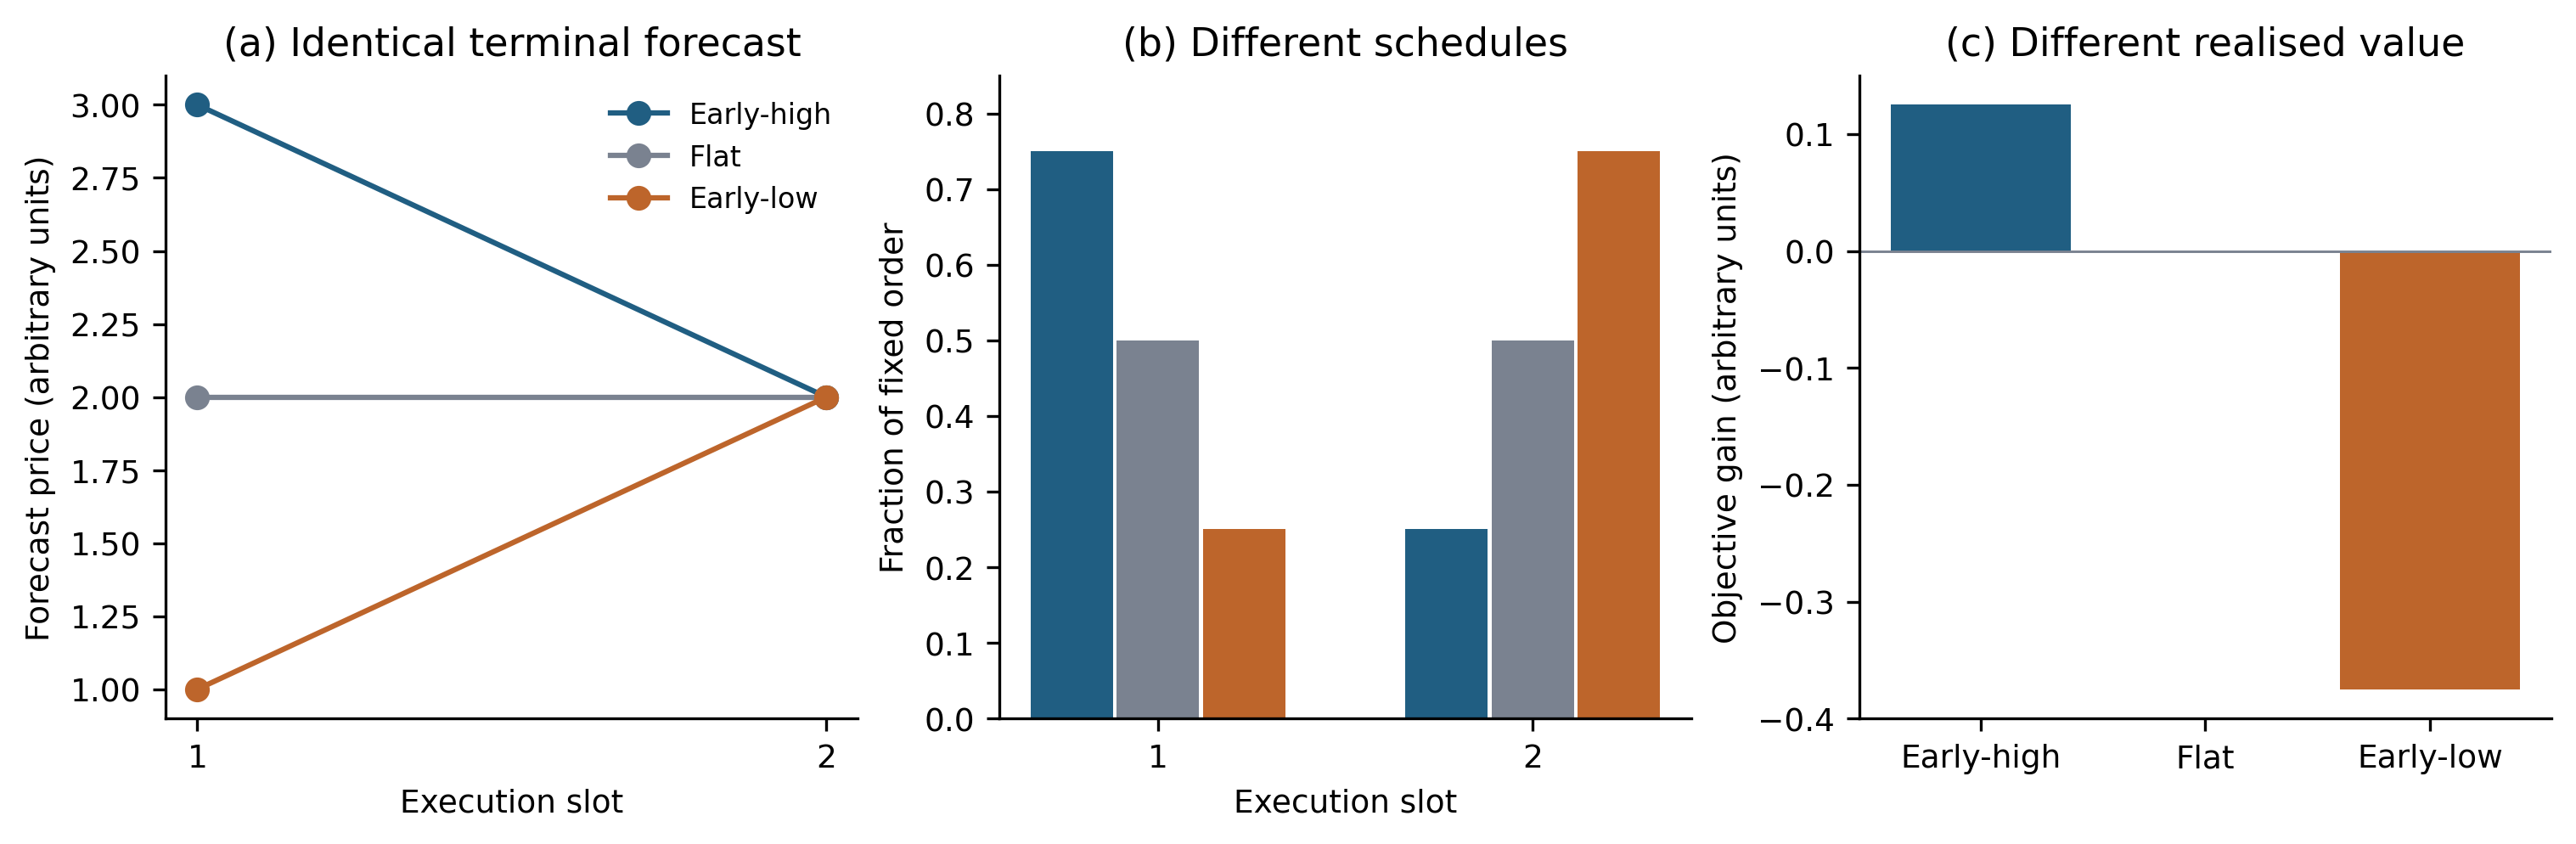
\includegraphics[width=\linewidth]{figures/fig01_endpoint_example.png}
\caption{Synthetic two-slot illustration, not observed market data. The three profiles share terminal forecast 2 but imply different schedules and gains. Prices and objective values are in arbitrary units.}
\label{fig:endpoint}
\end{figure}

\subsection{Exact timing-payoff and action-cost decomposition}
Set $\delta=u_1-u_0$ and mix the feasible schedules as $u(w)=u_0+w\delta$, where $0\leq w\leq1$. Convexity of $\mathcal U$ preserves nonnegativity and completion. The baseline-relative gain is
\begin{equation}
 G(w)=J_p(u_0)-J_p(u(w))=w(A-B)-w^2C,
 \label{eq:gain}
\end{equation}
with
\begin{align}
 A&=\delta^\top p,\qquad
 B=\nabla K(u_0)^\top\delta,\qquad
 C=\tfrac12\delta^\top H\delta.\label{eq:abc}
\end{align}
Equation~\eqref{eq:gain} follows by exact quadratic expansion. Baseline optimality gives $B\geq0$ for a direction toward any other feasible schedule. Also $C>0$ for nonzero $\delta$. If the baseline is interior to the simplex, its gradient is proportional to $\mathbf1$ and $B=0$. The full expression remains valid when constraints bind, so that simplification is not assumed generally.

The price term has a useful inventory interpretation. Define cumulative extra sales $D_j=\sum_{k\leq j}\delta_k$. Completion implies $D_N=0$, and discrete summation by parts gives
\begin{equation}
 A=-\sum_{j=1}^{N-1}D_j(p_{j+1}-p_j).\label{eq:inventory}
\end{equation}
Extra early sales benefit from subsequent declines and lose from subsequent increases. The price movement before the first executable slot cancels because both schedules still hold the full order then. This is exposure accounting, not identification of the hypothetical order's causal market impact.

For any positive exposure, gain is positive precisely when $A-B>wC$. Full exposure requires $A>B+C$. Therefore neither a correct terminal sign nor positive timing alignment alone establishes a worthwhile action. In the quadratic model, the linear payoff falls proportionally with attenuation, whereas curvature cost falls with its square. That relationship explains how a smaller deviation can improve the trade-off. It is conditional on a fixed pair of endpoint schedules; changing the impact coefficient and reoptimising changes the endpoints themselves.

\subsection{Historical exposure fitting}
A common coefficient fitted to historical episodes maximises
$w\overline{(A-B)}-w^2\overline C$. When $\overline C>0$, its solution is
\begin{equation}
 \widehat w_P=\operatorname{clip}_{[0,1]}
 \left\{\frac{\overline{(A-B)}}{2\overline C}\right\}.
 \label{eq:plugin}
\end{equation}
If $\overline C=0$, every direction is zero under the positive-definite Hessian and we select $\widehat w_P=0$. For $C_i>0$, define the realised target $z_i=(A_i-B_i)/(2C_i)$. Then
\[
 G_i(w)=C_i z_i^2-C_i(w-z_i)^2.
\]
Thus historical fitting is equivalent to curvature-weighted squared-error minimisation on the fixed feasible segment. It is not the mean of episode-level ratios, and the realised targets are unavailable at the time the episode's decision is made. Only preceding calibration observations may determine the implemented coefficient.

A lower-percentile variant replaces the historical aggregate ratio with the fifth percentile of day-resampled aggregate ratios before clipping. This is a conservative fitting heuristic, not predictive-coverage calibration or a theorem of safe future improvement. Such distinctions matter because formal decision-focused calibration and conformal coverage refer to different objects and assumptions \citep{liu2021,barber2023}.

Finally, mixing schedules is not generally identical to reoptimising a scaled forecast. With the two-slot cost above and forecast $(6,2)$, the full optimum is $(1,0)$. Half mixing with the baseline gives $(3/4,1/4)$, whereas the endpoint-preserving half-scaled forecast $(4,2)$ still optimises at $(1,0)$. Active-set changes break the global equivalence. Our policies mix the solved schedules, and all reported gains use that operation consistently.

\subsection{Data, episode construction and chronological design}
\label{sec:data}
The empirical illustration uses Binance spot BTCUSDT and ETHUSDT one-minute bars for January--August 2026 \citep{binance2026}. Sixteen monthly archives contain 699,840 observations. Before constructing episodes, the download procedure compares each archive with its published checksum and validates the complete minute grid. Checks cover calendar boundaries, microsecond timestamps, duplicates and gaps, close-time consistency, twelve-column structure, finite fields, positive prices, OHLC bounds, nonnegative volumes, integer trade counts and taker-buy volume bounded by total volume. All archives pass. These checks establish consistency of the downloaded bar records; they do not establish that an order could transact at the recorded open.

Each episode represents a hypothetical, normalised sell order completed over fifteen execution opportunities. Let $i$ denote a decision minute, selected at UTC minute offsets $5,35,\ldots,1415$. For total base volume $V_k$ and taker-buy base volume $V_k^B$, the observed signal is
\begin{equation}
 x_i=\frac{\sum_{k=i-5}^{i-1}(2V_k^B-V_k)}{\sum_{k=i-5}^{i-1}V_k},
 \label{eq:imbalance}
\end{equation}
with zero assigned when the denominator vanishes. Only five completed bars enter this signal. The execution-price vector uses opens at minutes $i+1,\ldots,i+15$, leaving a one-minute initial delay after the decision. Relative prices are $p_{ij}=10^4(P_{i+j}/P_i-1)$, where $P_i$ is the decision-minute open. Both the baseline and forecast-dependent schedule use the same denominator and realised prices. There are 48 episodes per asset per day, with nonoverlapping execution horizons. Nonoverlap removes shared execution bars within an asset; it does not imply independence across episodes or assets.

For each asset, a three-month window separates training, calibration and evaluation. The first window trains in January, calibrates in February and evaluates in March; subsequent windows advance by one month, ending with June training, July calibration and August evaluation. The resulting evaluation sample comprises 17,664 episodes across twelve asset--month windows and 184 calendar dates. Each evaluation-month policy uses only the two preceding months. Nevertheless, rolling windows share observations in different roles, and both assets experience common market conditions.

Figure~\ref{fig:rolling} summarises the calendar separation between forecast fitting, exposure fitting and evaluation.
\begin{figure}[htbp]\centering
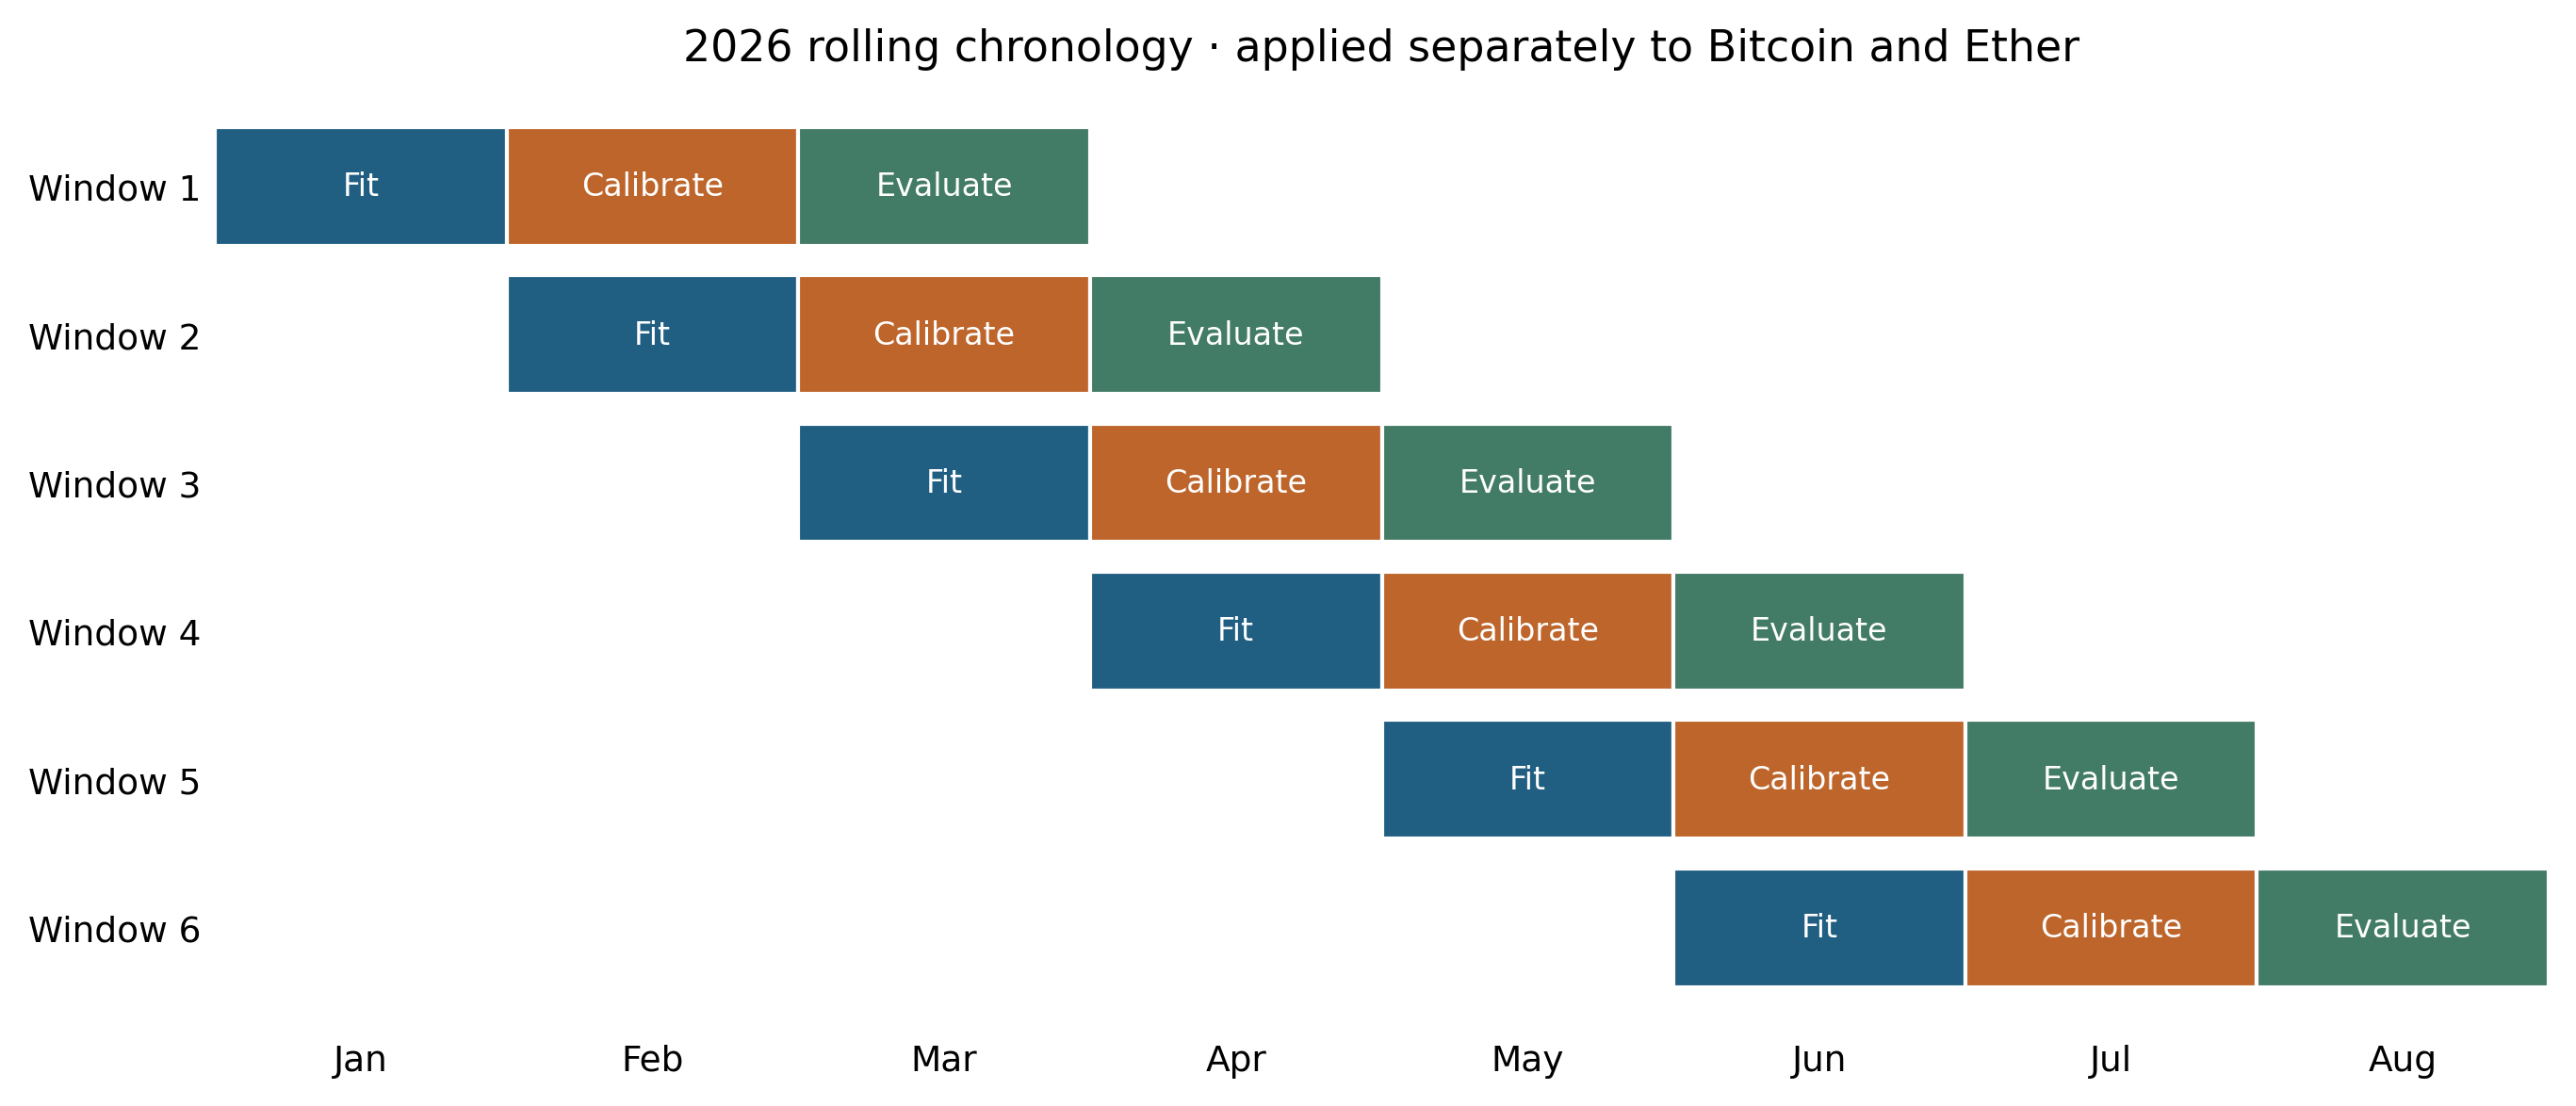
\includegraphics[width=\linewidth]{figures/fig02_rolling_design.png}
\caption{Rolling calendar design for each asset. Each evaluation month follows separate training and calibration months. Calendar ordering prevents within-window look-ahead, but does not make this retrospective extension prospectively preregistered or its entire sample previously unseen.}
\label{fig:rolling}
\end{figure}

The expanded design was recorded after examining an initial Bitcoin evaluation and before computing these expanded outcomes. Bitcoin's August evaluation overlaps that earlier analysis. The study is therefore a retrospective exploratory extension, not an independent confirmation or a prospective preregistration. This chronology motivates reporting every specified window, profile and cost scenario. No additional predictor search, horizon selection or outcome-dependent sample expansion is used in the extension.

\subsection{Forecast construction and matched-endpoint comparisons}
\label{sec:forecastconstruction}
Training fits fifteen ordinary least-squares regressions with intercept, one for each execution horizon. If $\widehat\beta_j$ is the slope on imbalance and $\bar x_{\mathrm{train}}$ its training mean, the forecast is
\begin{equation}
 \mu_{ij}=\widehat\beta_j(x_i-\bar x_{\mathrm{train}}).
\end{equation}
The unconditional fitted intercept is excluded deliberately, so the experiment concerns the estimated imbalance-dependent price profile. The slopes and centring value remain fixed during calibration and evaluation. This simple specification provides an auditable forecast input; it is not selected as the strongest available cryptocurrency predictor.

For each episode, three transformations of the learned profile preserve its final coordinate:
\begin{equation}
 \mu^{\mathrm{parallel}}_{ij}=\mu_{iN},\qquad
 \mu^{\mathrm{ramp}}_{ij}=\frac jN\mu_{iN},\qquad
 \mu^{\mathrm{mirror}}_{ij}=2\mu_{iN}-\mu_{ij},\quad N=15.
 \label{eq:profiles}
\end{equation}
The parallel profile contains no relative-price information across execution opportunities and must recover the no-signal baseline. It is therefore an analytical and numerical control. The ramp imposes a linear path connecting zero to the learned endpoint. The mirror reverses the learned profile's temporal contrasts around that endpoint. These constructions isolate the information discarded by an endpoint summary. In particular, the mirror is a deliberate counterfactual, not a separately estimated forecasting competitor.

Terminal root-mean-square error, directional hit rate and $R^2$ are identical across all four profiles episode by episode. The reported $R^2$ compares squared errors with a zero-return prediction:
\begin{equation}
 R^2_{\mathrm{terminal}}=1-
 \frac{\sum_i(p_{iN}-\mu_{iN})^2}{\sum_i p_{iN}^2}.
\end{equation}
Directional accuracy is the proportion for which forecast and realised terminal signs agree. These quantities remain useful descriptions of endpoint prediction, but they cannot rank the constructed schedules. Holding them fixed is the identification device, rather than a claim that all profiles are equally plausible models of the full price path.

\subsection{Policies, costs and outcome measurement}
\label{sec:policies}
Every profile is passed to the same nonnegative, unit-volume quadratic programme. The baseline minimises the same cost function without a price forecast. The primary specification is $\eta=2$ and $r=1$, with all six combinations of $\eta\in\{0.5,2,5\}$ and $r\in\{0,1\}$ retained as sensitivity checks. The impact parameter imposes a hypothetical monetary charge for concentrated execution. The inventory parameter expresses a preference for reducing remaining inventory; it is not an estimated variance or a realised cash payment. Neither coefficient is fitted to exchange-level fills or depth.

In addition to full exposure to each matched profile, three policies mix the learned schedule with the baseline: a fixed weight of $1/2$, the preceding month's plug-in weight $w_P$, and a lower-percentile weight $w_C$. The plug-in rule maximises mean calibration-month gain on $[0,1]$. For the latter rule, 2,000 resampled calibration days produce aggregate ratios $\overline{(A-B)}/(2\overline C)$; their fifth percentile is clipped to $[0,1]$. Coefficients are aggregated before taking the ratio, rather than averaging unstable episode-level ratios. The code selects zero for negligible aggregate curvature. Each resulting weight is fixed throughout the next evaluation month. The lower-percentile construction is a historical exposure rule, without a prospective coverage or safety guarantee.

The principal outcome is paired objective gain against the baseline, decomposed into price alignment, the baseline-gradient term and curvature cost. Monetary gain is also reported by removing the inventory penalty when scoring the same schedules. Thus it does not substitute a different monetary-optimal policy for the one actually selected. Shifted quantity, $\|u_1-u_0\|_1/2$, describes the fraction of the parent order reallocated between slots. A feasible equality-constrained solution is used when available, with a projected-gradient simplex solver otherwise; the maximum observed KKT residual is $1.29\times10^{-12}$.

\subsection{Aggregation and uncertainty}
\label{sec:uncertainty}
Pooled estimates weight episodes equally, so longer months contribute more observations. Equal asset--month means provide a weighting check. Evaluation intervals use 2,000 bootstrap draws of whole UTC days, retaining both assets together on each sampled date. This grouping preserves within-day serial and cross-asset co-movement. Fitted regressions, calibration weights and policies remain fixed during resampling; calibration and evaluation seeds are recorded in the reproducibility files.

These intervals summarise uncertainty conditional on the selected sample and fitted policies. They neither propagate the complete training and calibration procedure nor accommodate arbitrary dependence across days. No adjustment is made for the multiple profile, window and cost comparisons. Accordingly, interval exclusions of zero are descriptive evidence within the replay, not confirmatory discovery claims. This interpretation also separates uncertainty about the observed paired mean from the unmeasured difference between minute-open proxies and executable fills.

\FloatBarrier
\section{Results and Discussion}
\label{sec:results}
\subsection{Positive timing benefit does not cover the cost of acting}
The main result is a separation between gross timing information and its value after changing the schedule. Under the primary hypothetical cost specification, full exposure to the learned profile generates average price alignment of $0.00370$ basis points. Its additional curvature cost is $0.00805$ basis points, while the baseline-gradient term is zero to numerical precision. The resulting average objective gain is $-0.00436$ basis points, with a conditional 95\% interval of $[-0.00829,-0.00047]$. The forecast-induced reallocation aligns positively with subsequent price changes on average, but that benefit does not cover the model's charge for departing from the baseline.

\begin{table}[htbp]
\centering\small
\caption{Matched endpoint forecasts and primary execution outcomes. All quantities are basis points under $\eta=2,r=1$. Price alignment and curvature are the terms in the gain decomposition; intervals are conditional day-bootstrap summaries. Parallel gains are analytically zero, with raw absolute mean numerical residuals below $1.5\times10^{-14}$.}
\label{tab:profiles}
\resizebox{\linewidth}{!}{\begin{tabular}{lrrr}
\toprule
Profile & Price alignment & Curvature & Net gain [95\% interval] \\
\midrule
Parallel & 0.00000 & 0.00000 & 0.00000 [0.00000, 0.00000] \\
Learned & 0.00370 & 0.00805 & -0.00436 [-0.00829, -0.00047] \\
Ramp & 0.00339 & 0.00434 & -0.00095 [-0.00520, 0.00285] \\
Mirror & -0.00370 & 0.00805 & -0.01175 [-0.01537, -0.00832] \\
\bottomrule
\end{tabular}
}
\end{table}

\begin{figure}[htbp]\centering
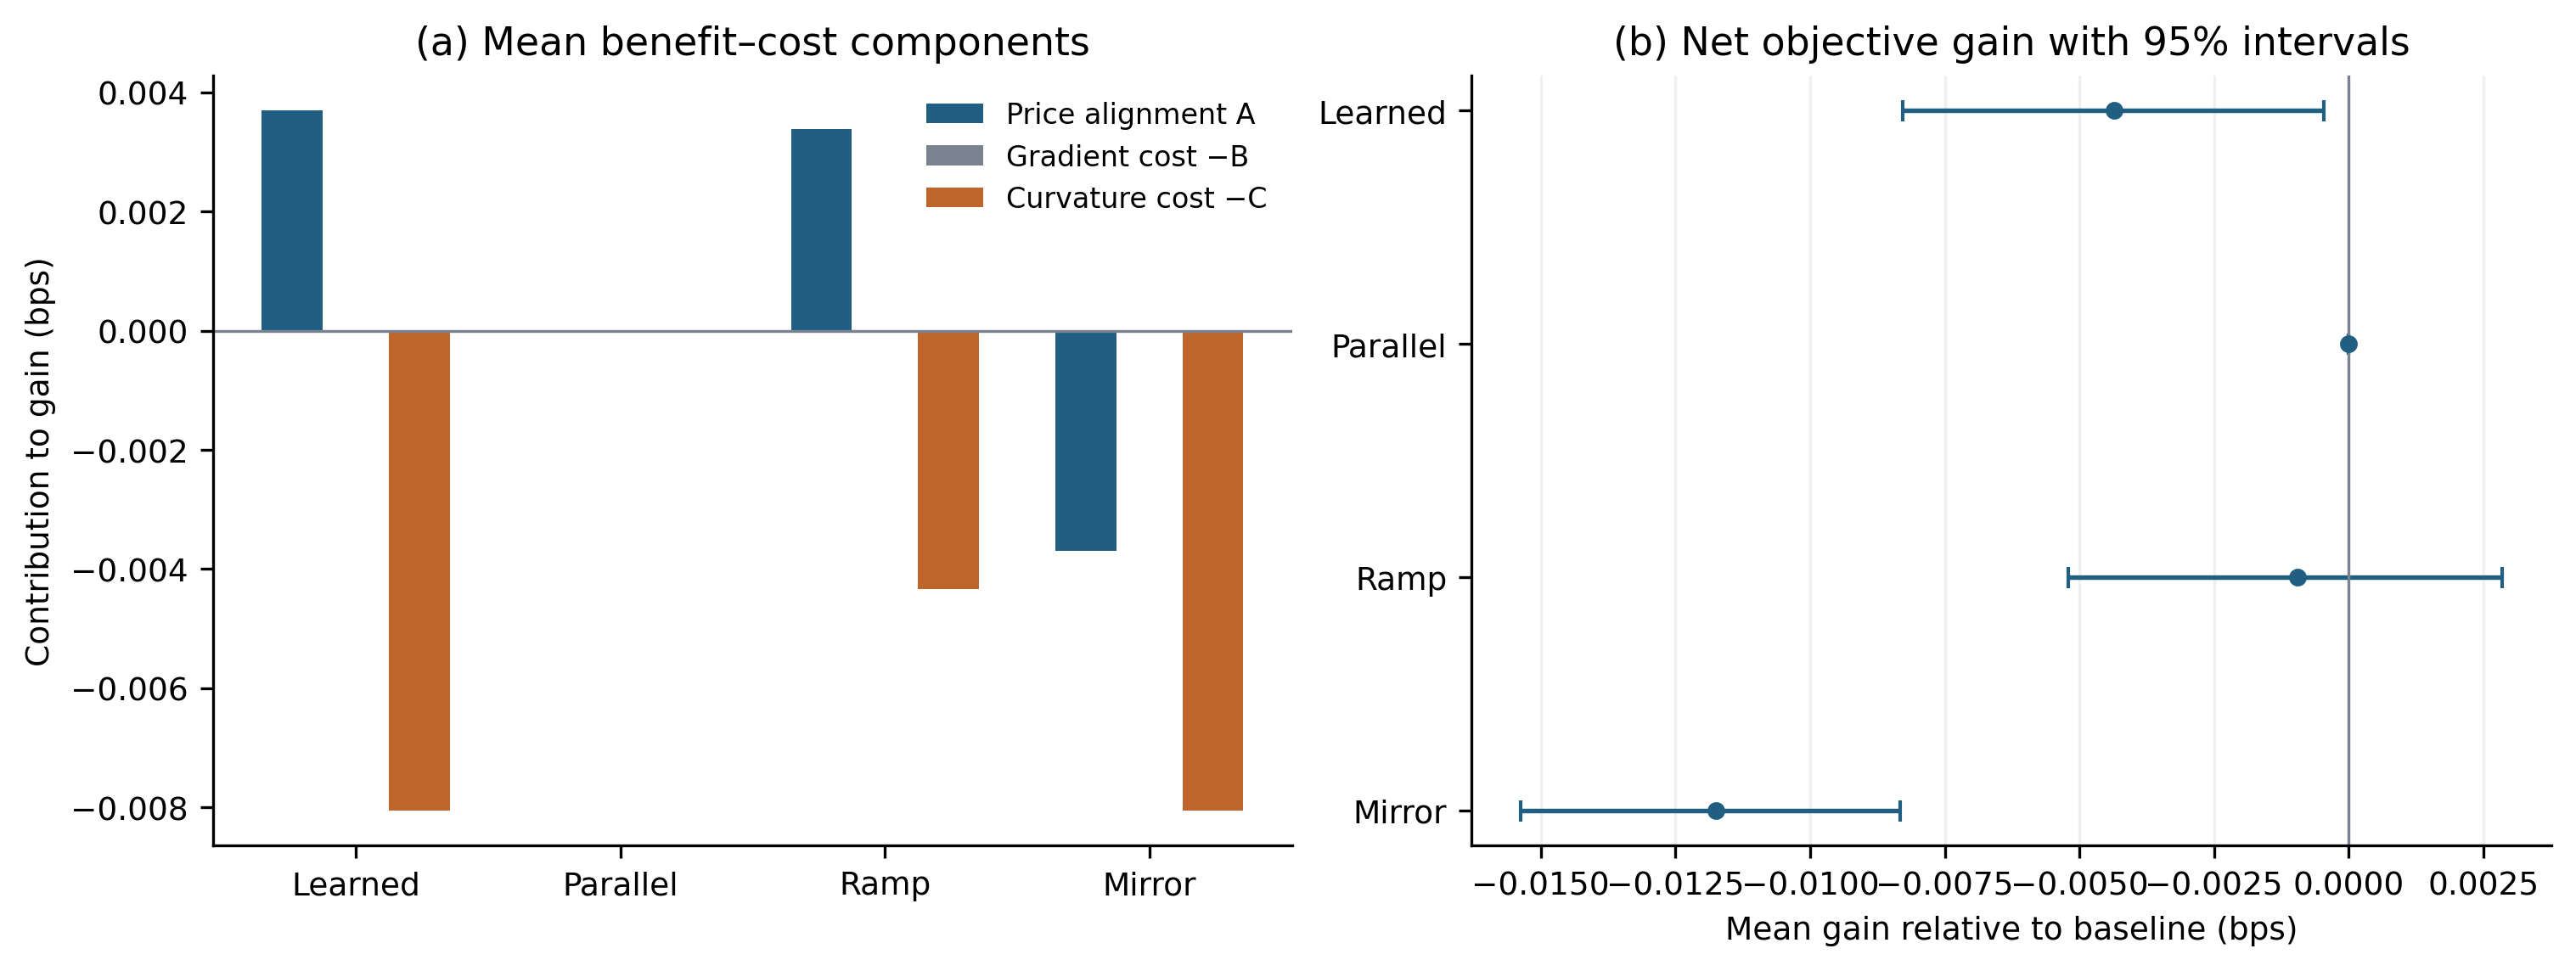
\includegraphics[width=\linewidth]{figures/fig03_benefit_cost.png}
\caption{Primary benefit--cost decomposition and matched-profile gains. Panel (a) reports episode-weighted $A$, $-B$ and $-C$, which sum to objective gain; $B$ is numerically zero. Panel (b) shows conditional 95\% calendar-day bootstrap intervals, resampling both assets jointly. The mirror is a diagnostic counterfactual.}
\label{fig:benefitcost}
\end{figure}

Figure~\ref{fig:benefitcost} displays this decomposition alongside the net outcomes. The first-order baseline term vanishes because the primary baseline lies in the interior of the nonnegative simplex. Its cost gradient is therefore constant across coordinates and orthogonal to feasible schedule changes. The remaining comparison has a direct economic meaning: the positive linear price benefit competes with a quadratic cost of shifting the order. Average shifted quantity is approximately $1.82\%$ of the parent order. Even this relatively small reallocation can be excessive when predictive timing information is weak.

The magnitude matters as well as the sign. The full-exposure loss is approximately $0.44$ parts per million of reference notional within the assumed objective. It would be misleading to turn this statistically distinguishable model difference into a claim of commercially material losses. The evidence supports a diagnostic distinction---positive timing alignment is insufficient for beneficial execution---at a small model-based scale.

\subsection{Identical endpoint scores conceal different schedule outcomes}
Table~\ref{tab:profiles} holds every terminal forecast fixed while changing the within-horizon profile. The parallel profile reproduces the baseline, as required by price-level invariance. The ramp has mean gain $-0.00095$ basis points, with interval $[-0.00520,0.00285]$. The mirror has mean gain $-0.01175$ basis points, with interval $[-0.01537,-0.00832]$. These differences cannot be attributed to changes in endpoint root-mean-square error, hit rate or $R^2$: those predictions and scores are identical by construction.

For the primary specification, the learned and mirrored schedules incur the same average curvature cost, approximately $0.00805$ basis points. Their price-alignment terms have opposite signs, approximately $0.00370$ and $-0.00370$. Reversing temporal contrasts therefore reverses gross timing benefit while retaining the same endpoint prediction. The ramp induces a smaller curvature cost, approximately $0.00434$ basis points, against price alignment of $0.00339$. Its smaller net loss illustrates that a less expensive response can outperform a more detailed estimated path without improving terminal accuracy.

The paired learned-minus-ramp difference is $-0.00341$ basis points, interval $[-0.00770,0.00101]$. The learned profile is consequently not demonstrably superior to this restricted construction. Its learned-minus-mirror difference is $0.00739$ basis points, interval $[0.00076,0.01468]$. The latter result verifies the importance of temporal orientation in this replay, but is not a competitive forecasting victory: the mirror was designed to reverse that orientation. The diagnostic's contribution rests on exposing an omission in endpoint evaluation, rather than on choosing a winning profile.

\subsection{Window heterogeneity and weak endpoint predictability}
Table~\ref{tab:windows} reports all twelve asset--month windows. Terminal hit rates range from $47.9\%$ to $52.6\%$, and terminal $R^2$ values remain close to zero. The simple imbalance specification thus provides limited endpoint predictive evidence in this sample. Full learned exposure produces positive objective gains in five windows and negative gains in seven. The pooled negative result is not a statement that every month or both assets at every date behave identically.

\begin{table}[htbp]
\centering\small
\caption{All primary evaluation windows. Gains are objective basis points; $w_P$ and $w_C$ are fitted on the preceding month. Terminal diagnostics apply identically to all matched profiles. All dates are in 2026.}
\label{tab:windows}
\resizebox{\linewidth}{!}{\begin{tabular}{llrrrrrr}
\toprule
Asset & Month & Hit rate & Terminal $R^2$ & Learned & Ramp & $w_P$ & $w_C$ \\
\midrule
BTC & 03 & 51.9\% & -0.00005 & 0.00184 & 0.00024 & 0.000 & 0.000 \\
BTC & 04 & 49.0\% & -0.00452 & -0.03025 & -0.01944 & 0.000 & 0.000 \\
BTC & 05 & 52.6\% & -0.00037 & -0.00648 & -0.00086 & 0.058 & 0.000 \\
BTC & 06 & 48.8\% & -0.00022 & 0.00003 & 0.00168 & 0.000 & 0.000 \\
BTC & 07 & 50.0\% & 0.00007 & -0.00035 & 0.00001 & 0.520 & 0.000 \\
BTC & 08 & 49.5\% & -0.00127 & 0.00488 & -0.00889 & 0.000 & 0.000 \\
ETH & 03 & 50.5\% & -0.00046 & -0.00535 & -0.00224 & 0.000 & 0.000 \\
ETH & 04 & 47.9\% & -0.00006 & -0.02624 & -0.00140 & 0.049 & 0.000 \\
ETH & 05 & 50.5\% & 0.00034 & -0.00809 & 0.00434 & 0.000 & 0.000 \\
ETH & 06 & 48.4\% & -0.00002 & -0.00072 & 0.00273 & 0.620 & 0.000 \\
ETH & 07 & 51.1\% & 0.00189 & 0.00695 & 0.00692 & 0.824 & 0.000 \\
ETH & 08 & 50.7\% & 0.00070 & 0.01023 & 0.00508 & 0.674 & 0.000 \\
\bottomrule
\end{tabular}
}
\end{table}

\begin{figure}[htbp]\centering
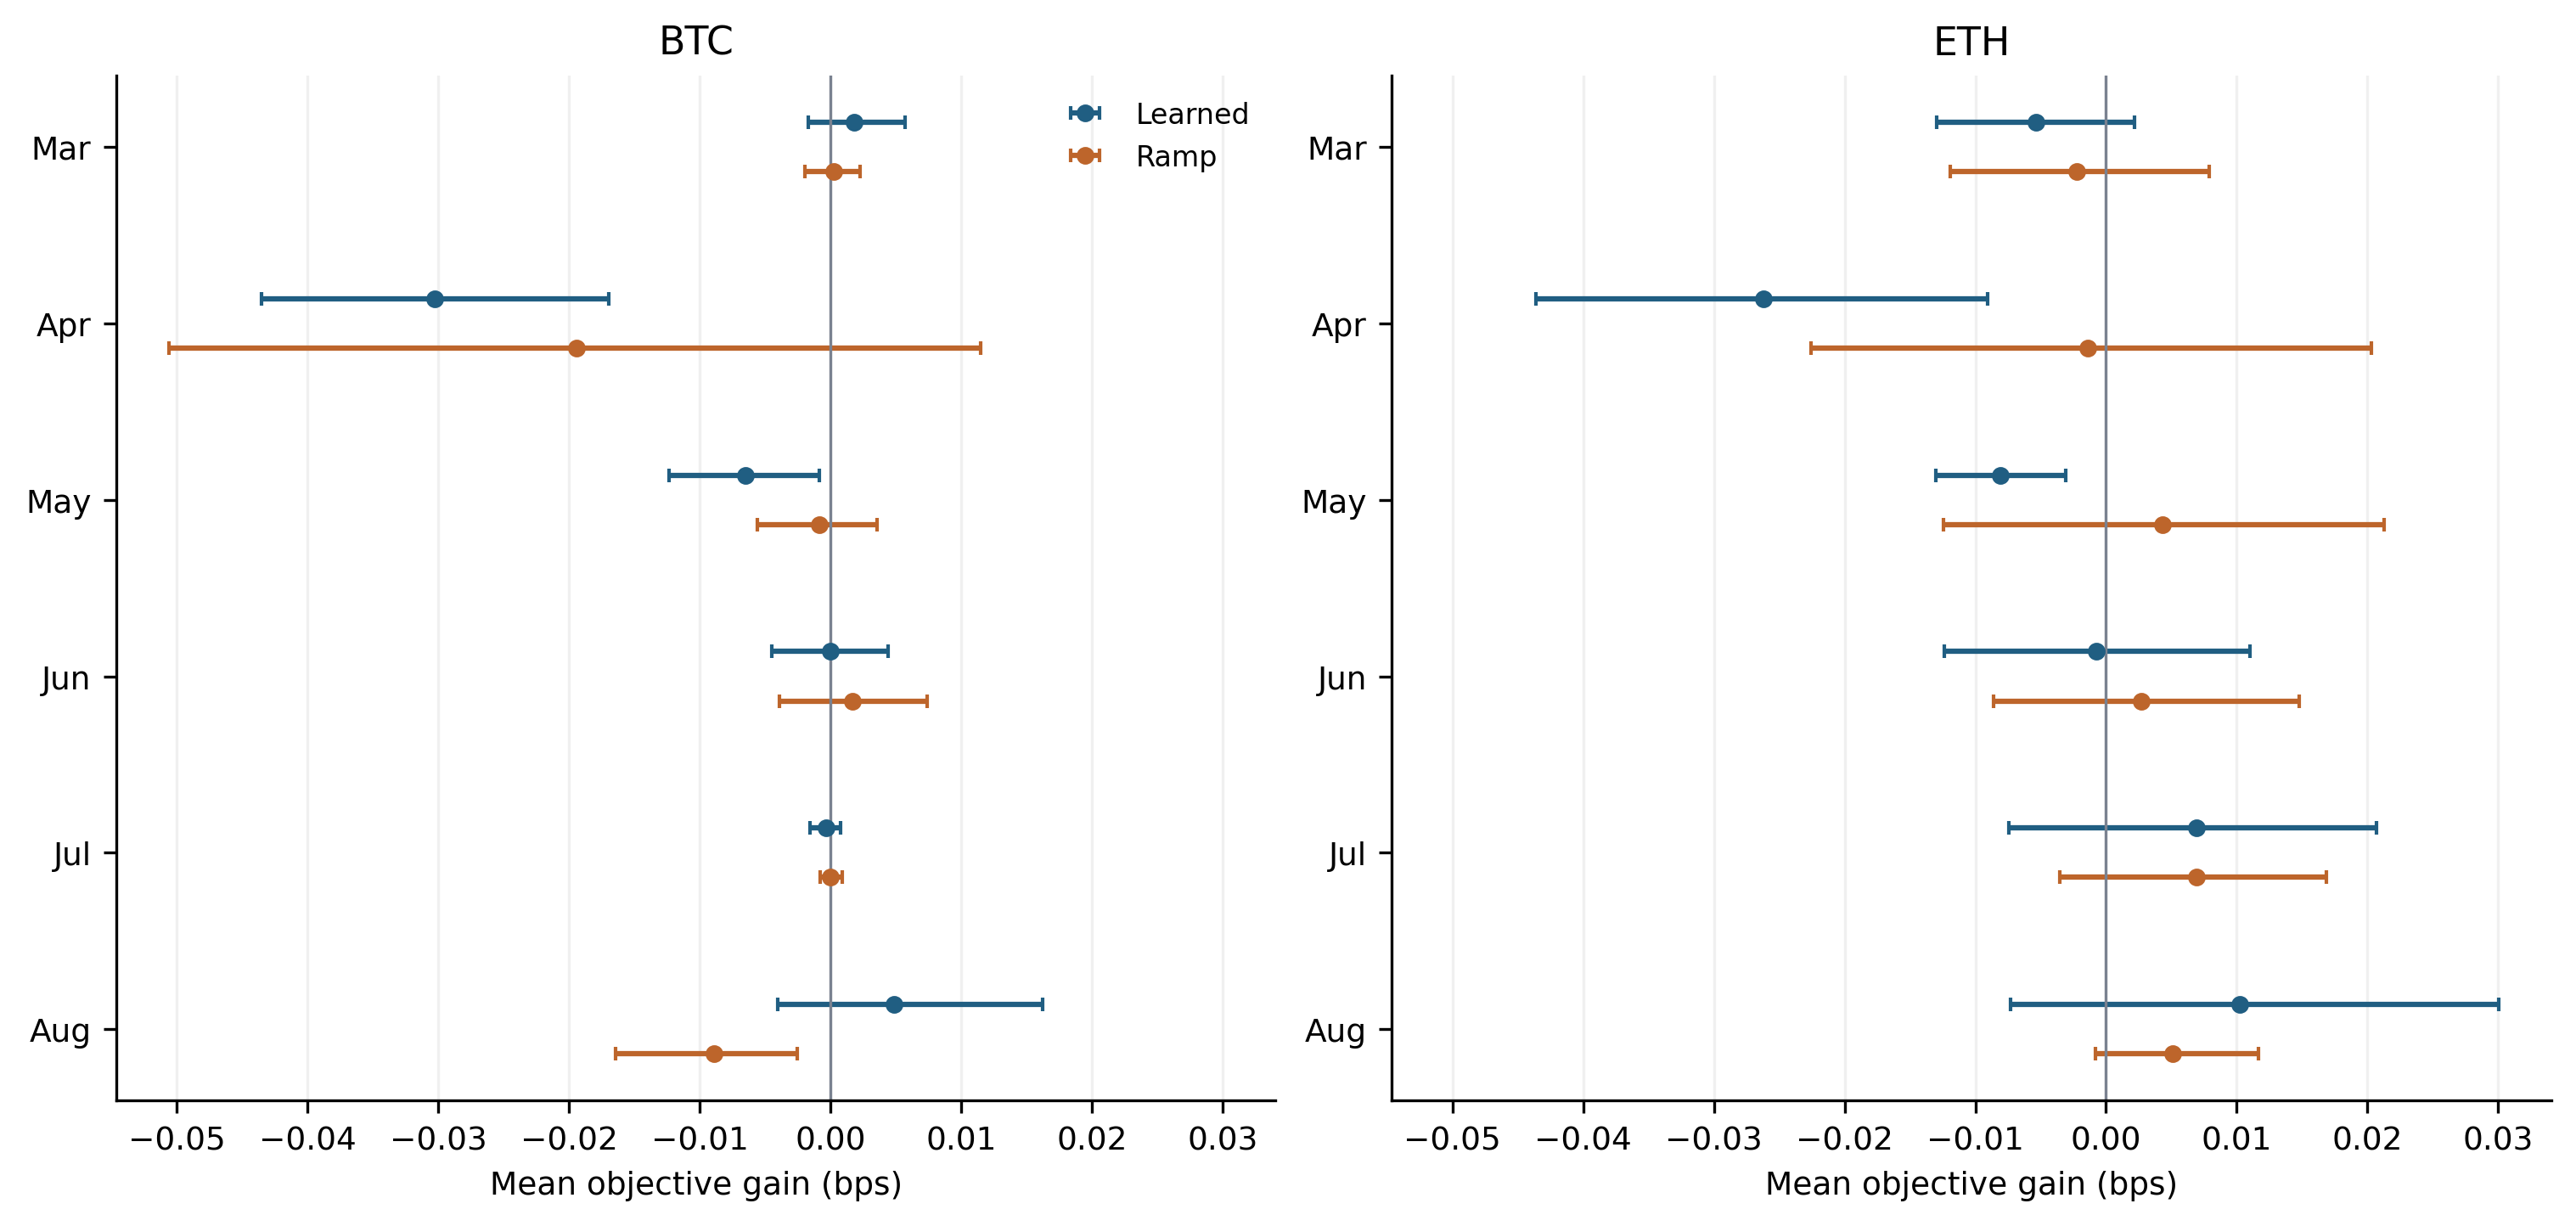
\includegraphics[width=\linewidth]{figures/fig04_monthly_gains.png}
\caption{All twelve primary asset--month evaluations. Learned and ramp points show full-exposure mean objective gains, with stored 95\% within-window calendar-day bootstrap intervals. Intervals condition on fitted forecasts, and overlapping windows are not independent replications.}
\label{fig:monthlygains}
\end{figure}

Figure~\ref{fig:monthlygains} shows the dispersion and within-window intervals. April contributes relatively large negative learned gains for both Bitcoin ($-0.03025$ basis points) and Ether ($-0.02624$). The final two Ether windows instead have positive gains of $0.00695$ and $0.01023$ basis points. Bitcoin's August learned gain is also positive, at $0.00488$ basis points. These changes indicate temporal heterogeneity in the relationship between fitted price profiles and realised timing payoffs. The design does not identify a causal market-regime explanation for that heterogeneity.

Endpoint diagnostics do not resolve the schedule comparison. Bitcoin in May records the highest reported hit rate, $52.6\%$, but its learned schedule loses $0.00648$ basis points against the baseline. Ether in May has positive terminal $R^2$ but a learned gain of $-0.00809$ basis points; its ramp gain is positive at $0.00434$. These are illustrative rows from the complete table, not selected tests of a general relationship between hit rates and gains. More decisively, each row's endpoint statistics are shared by the learned, ramp, mirror and parallel profiles despite their different decisions.

Equal weighting of the twelve asset--month means gives a learned gain of $-0.00446$ basis points, close to the episode-weighted $-0.00436$. Unequal month lengths therefore do not explain the pooled sign. Both summaries still describe overlapping rolling windows from one exchange and one eight-month input period; changing aggregation does not create independent evidence.

An additional ex post influence diagnostic recomputes the primary mean after omitting each evaluation month from both assets, without refitting forecasts or weights (Figure~\ref{fig:influence}). Omitting April changes the learned mean to $+0.00030$ basis points; all other single-month omissions retain a negative mean. The pooled negative sign is therefore sensitive to April's inclusion, despite its persistence across the specified cost grid. This display diagnoses concentration rather than defining a preferable subsample: the headline estimate retains every month, and no inferential interval is attached to the omission exercise.

\begin{figure}[htbp]\centering
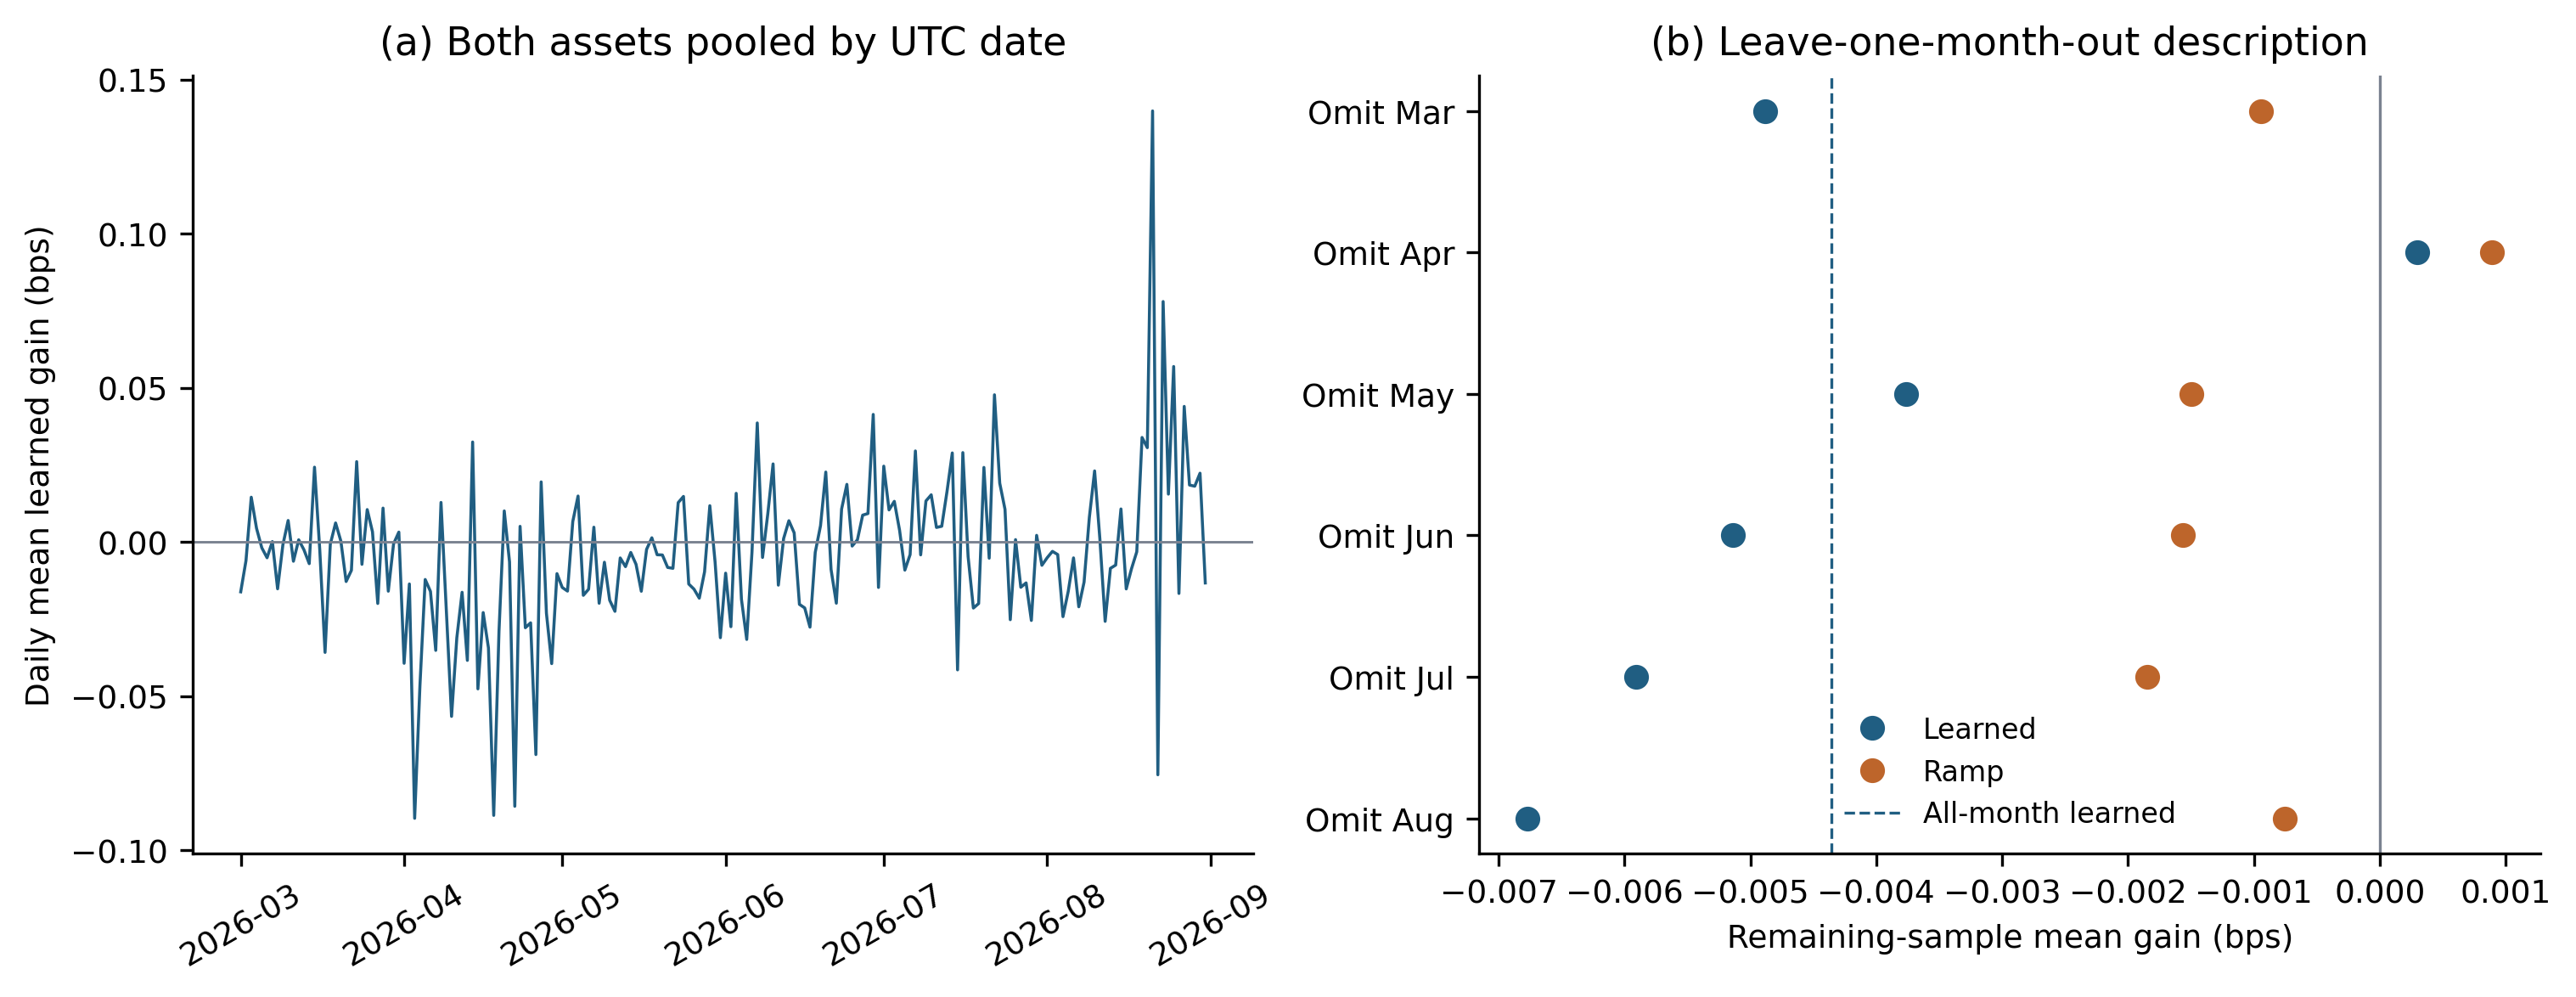
\includegraphics[width=\linewidth]{figures/fig08_descriptive_influence.png}
\caption{Additional ex post descriptive influence diagnostics from unchanged primary episodes. Panel (a) averages learned gains across both assets by UTC date. Panel (b) omits one evaluation month from both assets and recomputes the remaining mean; the dashed line is the full-sample mean. No forecasts or policies are refitted, and no confidence intervals or sample-selection recommendation are implied.}
\label{fig:influence}
\end{figure}

\subsection{Exposure fitting: partial improvement without a reliable advantage}
Table~\ref{tab:calibrated} compares ways of limiting the learned profile's influence. Half exposure yields mean objective gain $-0.00017$ basis points, with interval $[-0.00196,0.00171]$. Its movement towards zero follows the benefit--cost decomposition: halving exposure halves the linear timing term but quarters curvature cost. This improvement relative to full exposure is compatible with positive but weak timing information. It does not establish a positive expected execution saving.

\begin{table}[htbp]
\centering\small
\caption{Primary learned-profile exposure policies. Monetary gain drops the inventory-preference term when evaluating the same schedules. All gains are basis points; intervals refer to objective gain.}
\label{tab:calibrated}
\resizebox{\linewidth}{!}{\begin{tabular}{lrrr}
\toprule
Exposure policy & Objective gain & 95\% interval & Monetary gain \\
\midrule
Learned & -0.00436 & [-0.00829, -0.00047] & -0.00411 \\
Half learned & -0.00017 & [-0.00196, 0.00171] & -0.00007 \\
Plug-in & 0.00124 & [-0.00035, 0.00285] & 0.00125 \\
Lower-percentile & 0.00000 & [0.00000, 0.00000] & 0.00000 \\
\bottomrule
\end{tabular}
}
\end{table}

The plug-in rule selects positive weights in six of twelve windows and has pooled gain $0.00124$ basis points, interval $[-0.00035,0.00285]$. Its point estimate is favourable, but its conditional interval includes zero. The estimated weights vary markedly: Bitcoin's positive weights occur in May and July, while Ether's occur in April and June--August. Prior-month fitting therefore sometimes retains forecast exposure and sometimes rejects it. The data do not demonstrate a stable gain from this policy across future periods.

\begin{figure}[htbp]\centering
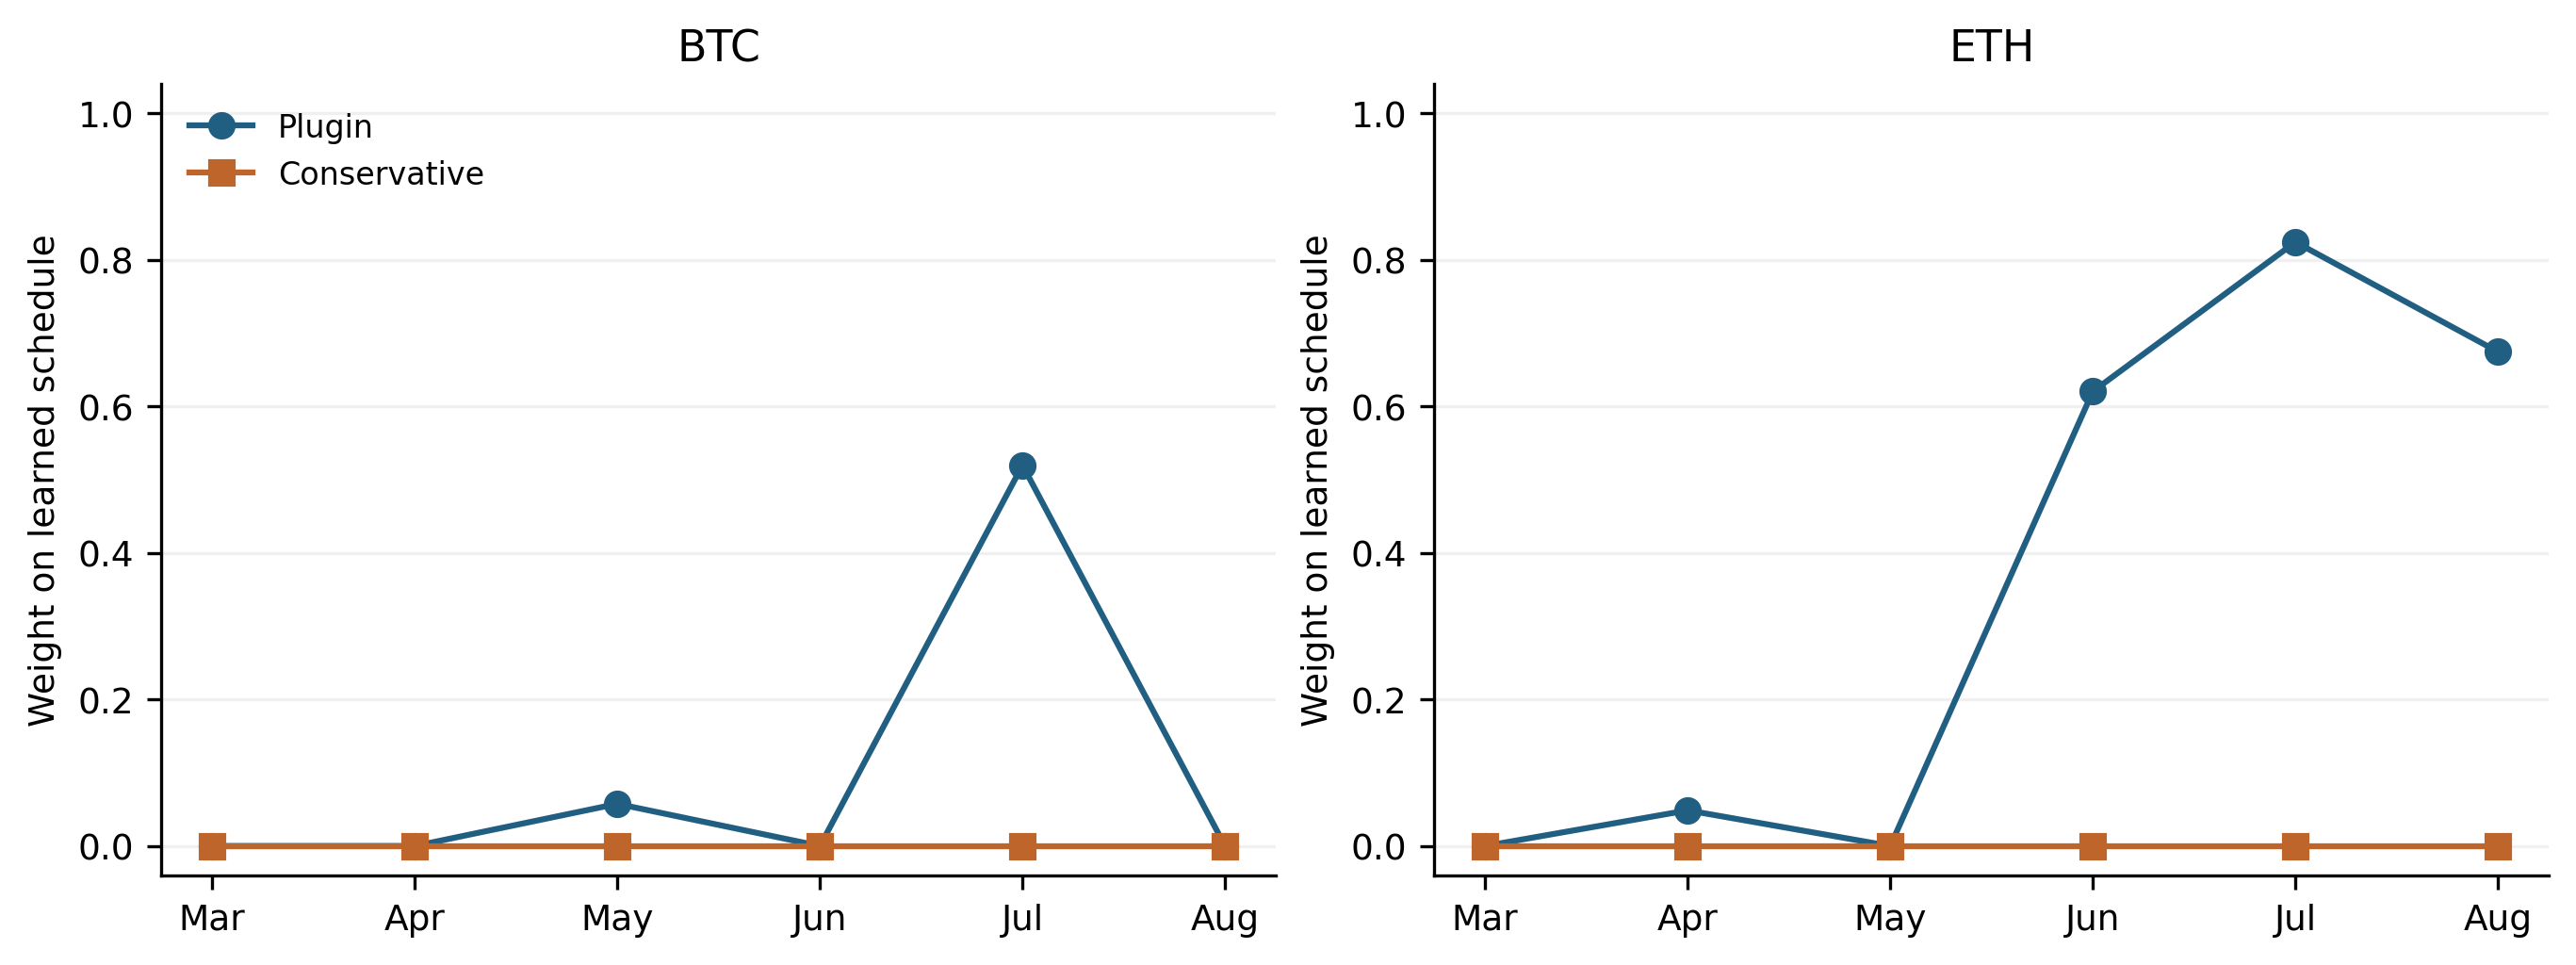
\includegraphics[width=\linewidth]{figures/fig05_calibrated_exposure.png}
\caption{Primary schedule-mixture weights fitted on the preceding calibration month. Plug-in weights are positive in six windows; lower-percentile weights are zero throughout. These weights are determined before each evaluation month within the retrospective design.}
\label{fig:exposure}
\end{figure}

Figure~\ref{fig:exposure} makes the variation in fitted exposure explicit. The lower-percentile rule selects zero in every window. Its realised paired gains are identically zero because its schedule equals the baseline, so its degenerate interval expresses policy identity. It does not imply certainty about future market conditions or the baseline's own costs. In this sample, the rule avoids the full-exposure loss, but it contributes no action beyond unconditional abstention. Accordingly, this result cannot establish superior calibration, robustness or safety.

Evaluating the pooled quadratic curve after observing all outcomes helps interpret these comparisons. Positive linear benefit creates a region in which smaller exposure has a positive retrospective mean gain; curvature eventually dominates as exposure increases. Any maximum computed from that evaluation curve is hindsight information. It is distinct from the monthly weights fitted on preceding data and is not reported as an implementable additional policy.

\subsection{Sensitivity to assumed impact and inventory preferences}
Full learned exposure has a negative pooled point estimate under every specified cost scenario (Table~\ref{tab:sensitivity}). At $\eta=0.5,r=0$, the estimate is $-0.01420$ basis points and its interval includes zero. Adding the inventory preference at the same impact coefficient gives $-0.01562$. At $\eta=5$, the losses are smaller, approximately $-0.00171$ and $-0.00172$ for $r=0$ and $r=1$. The remaining intervals exclude zero under the stated conditional resampling procedure.

\begin{table}[htbp]
\centering\small
\caption{All six hypothetical cost specifications. The same observations underlie each scenario, so these are sensitivity comparisons rather than independent replications. Full policy results are retained in the machine-readable output.}
\label{tab:sensitivity}
\resizebox{\linewidth}{!}{\begin{tabular}{rrrrr}
\toprule
$\eta$ & $r$ & Learned gain & 95\% interval & Plug-in gain \\
\midrule
0.5 & 0 & -0.01420 & [-0.02929, 0.00141] & 0.00533 \\
0.5 & 1 & -0.01562 & [-0.02908, -0.00193] & 0.00409 \\
2 & 0 & -0.00427 & [-0.00833, -0.00024] & 0.00133 \\
2 & 1 & -0.00436 & [-0.00829, -0.00047] & 0.00124 \\
5 & 0 & -0.00171 & [-0.00333, -0.00010] & 0.00053 \\
5 & 1 & -0.00172 & [-0.00333, -0.00014] & 0.00052 \\
\bottomrule
\end{tabular}
}
\end{table}

\begin{figure}[htbp]\centering
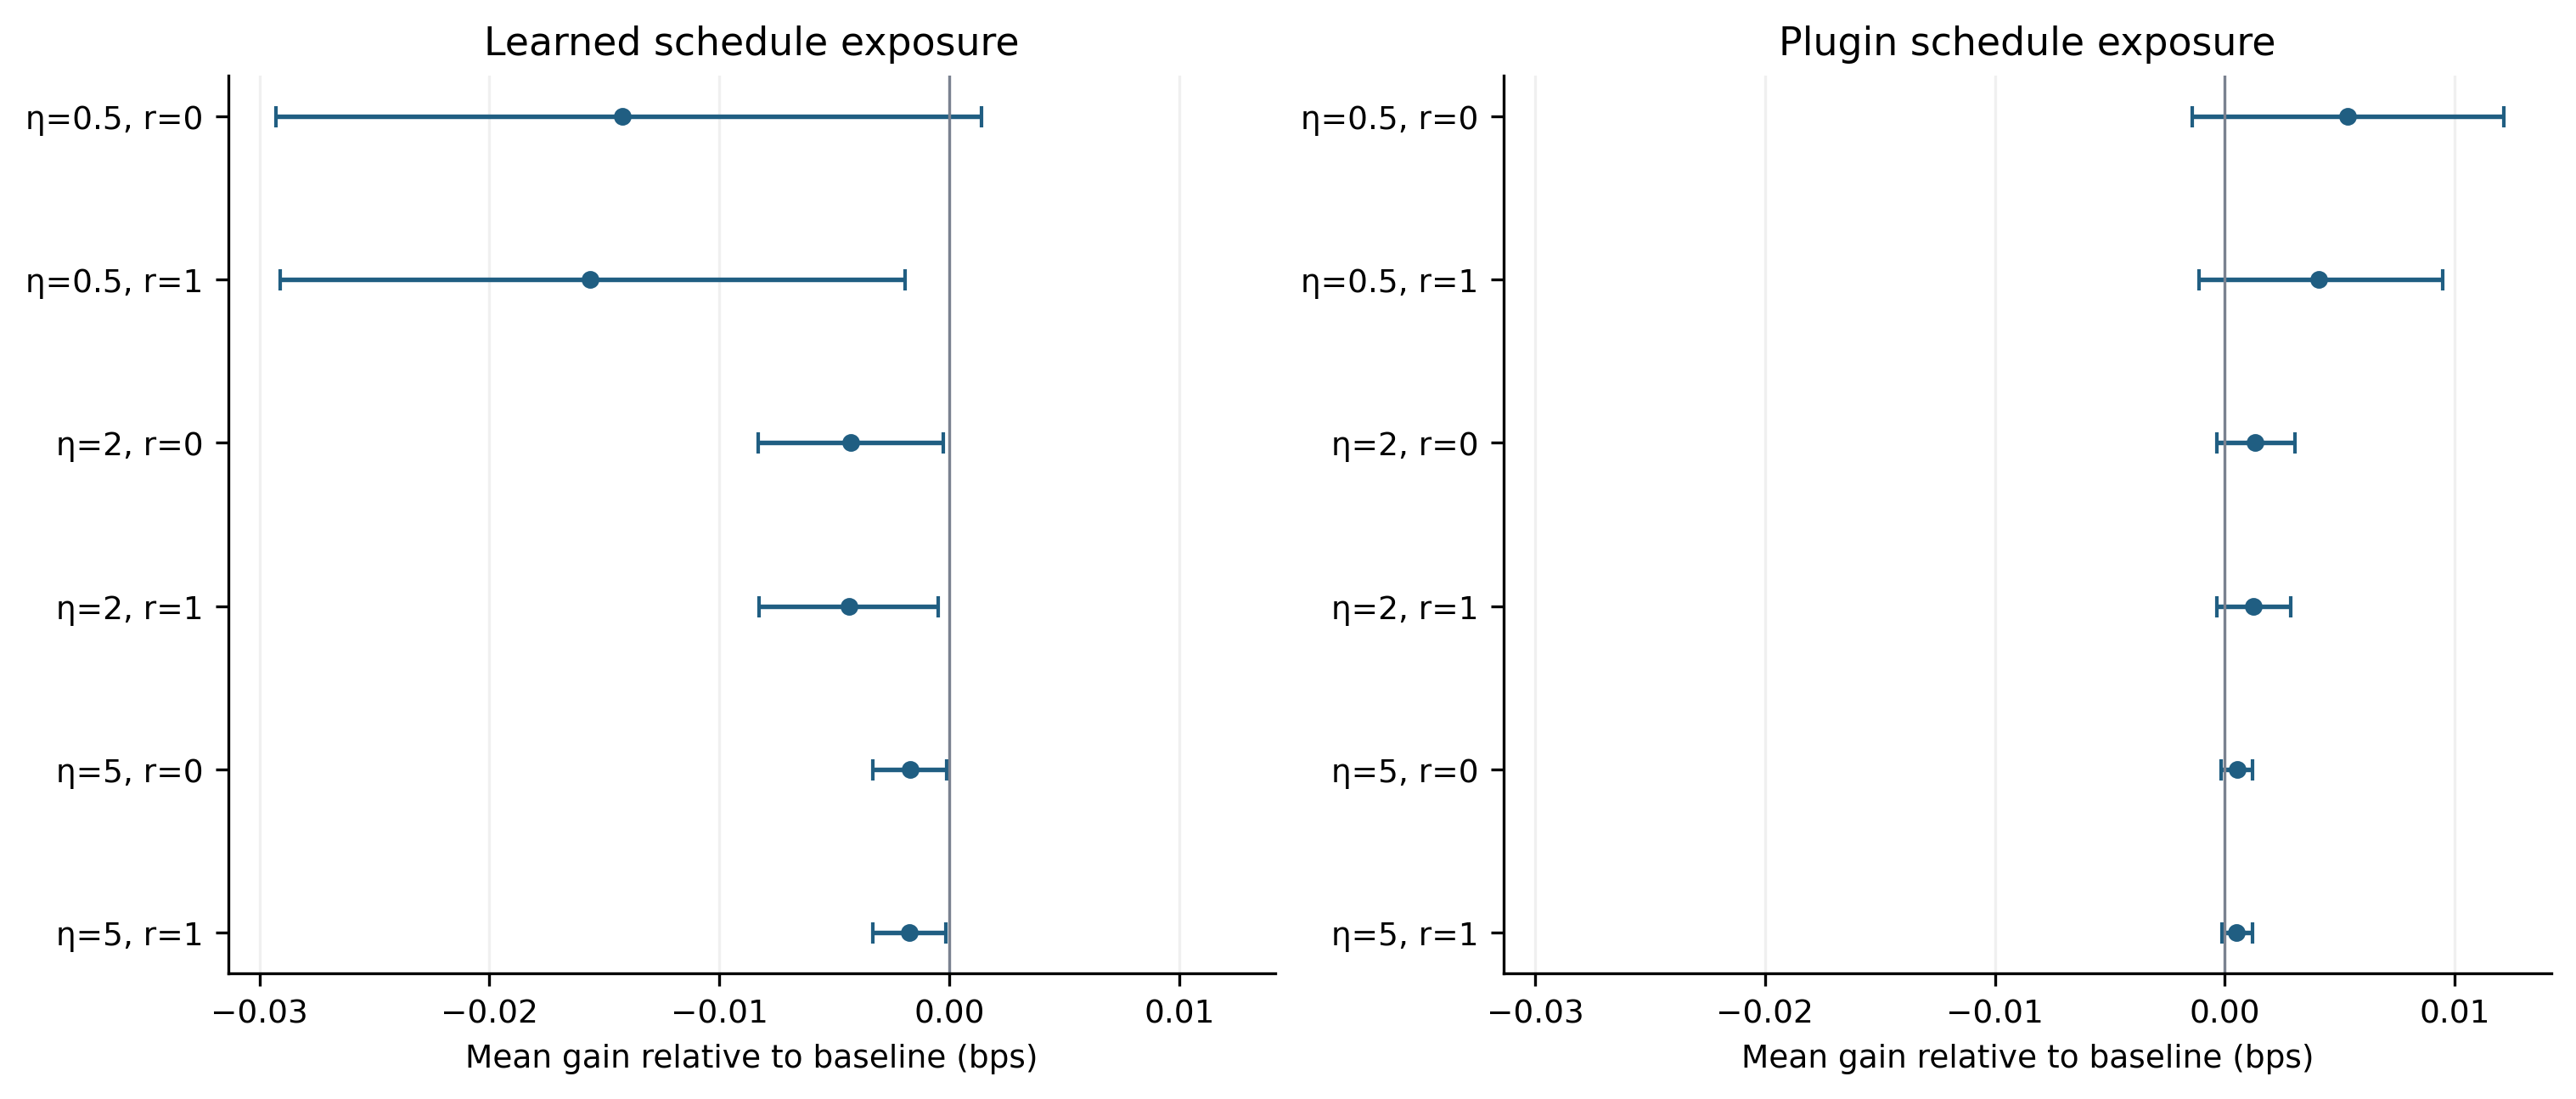
\includegraphics[width=\linewidth]{figures/fig07_cost_sensitivity.png}
\caption{All six specified cost scenarios for full learned exposure and the prior-month plug-in mixture. Points and conditional 95\% day-bootstrap intervals come from the unchanged analysis. Impact and inventory coefficients are assumed rather than estimated from exchange execution.}
\label{fig:sensitivity}
\end{figure}

Figure~\ref{fig:sensitivity} also displays plug-in intervals across the full cost grid. Increasing the impact coefficient changes the optimised schedule itself. Larger penalties discourage reallocation, so the smaller loss at high $\eta$ is not evidence that greater real-world trading costs improve an unchanged strategy. It reflects the response of a cost-aware optimiser to a stronger assumed penalty. The six-scenario grid demonstrates persistence of the negative full-exposure point estimate over this specified range; it cannot validate the coefficients as plausible costs for a particular parent-order size.

\begin{figure}[htbp]\centering
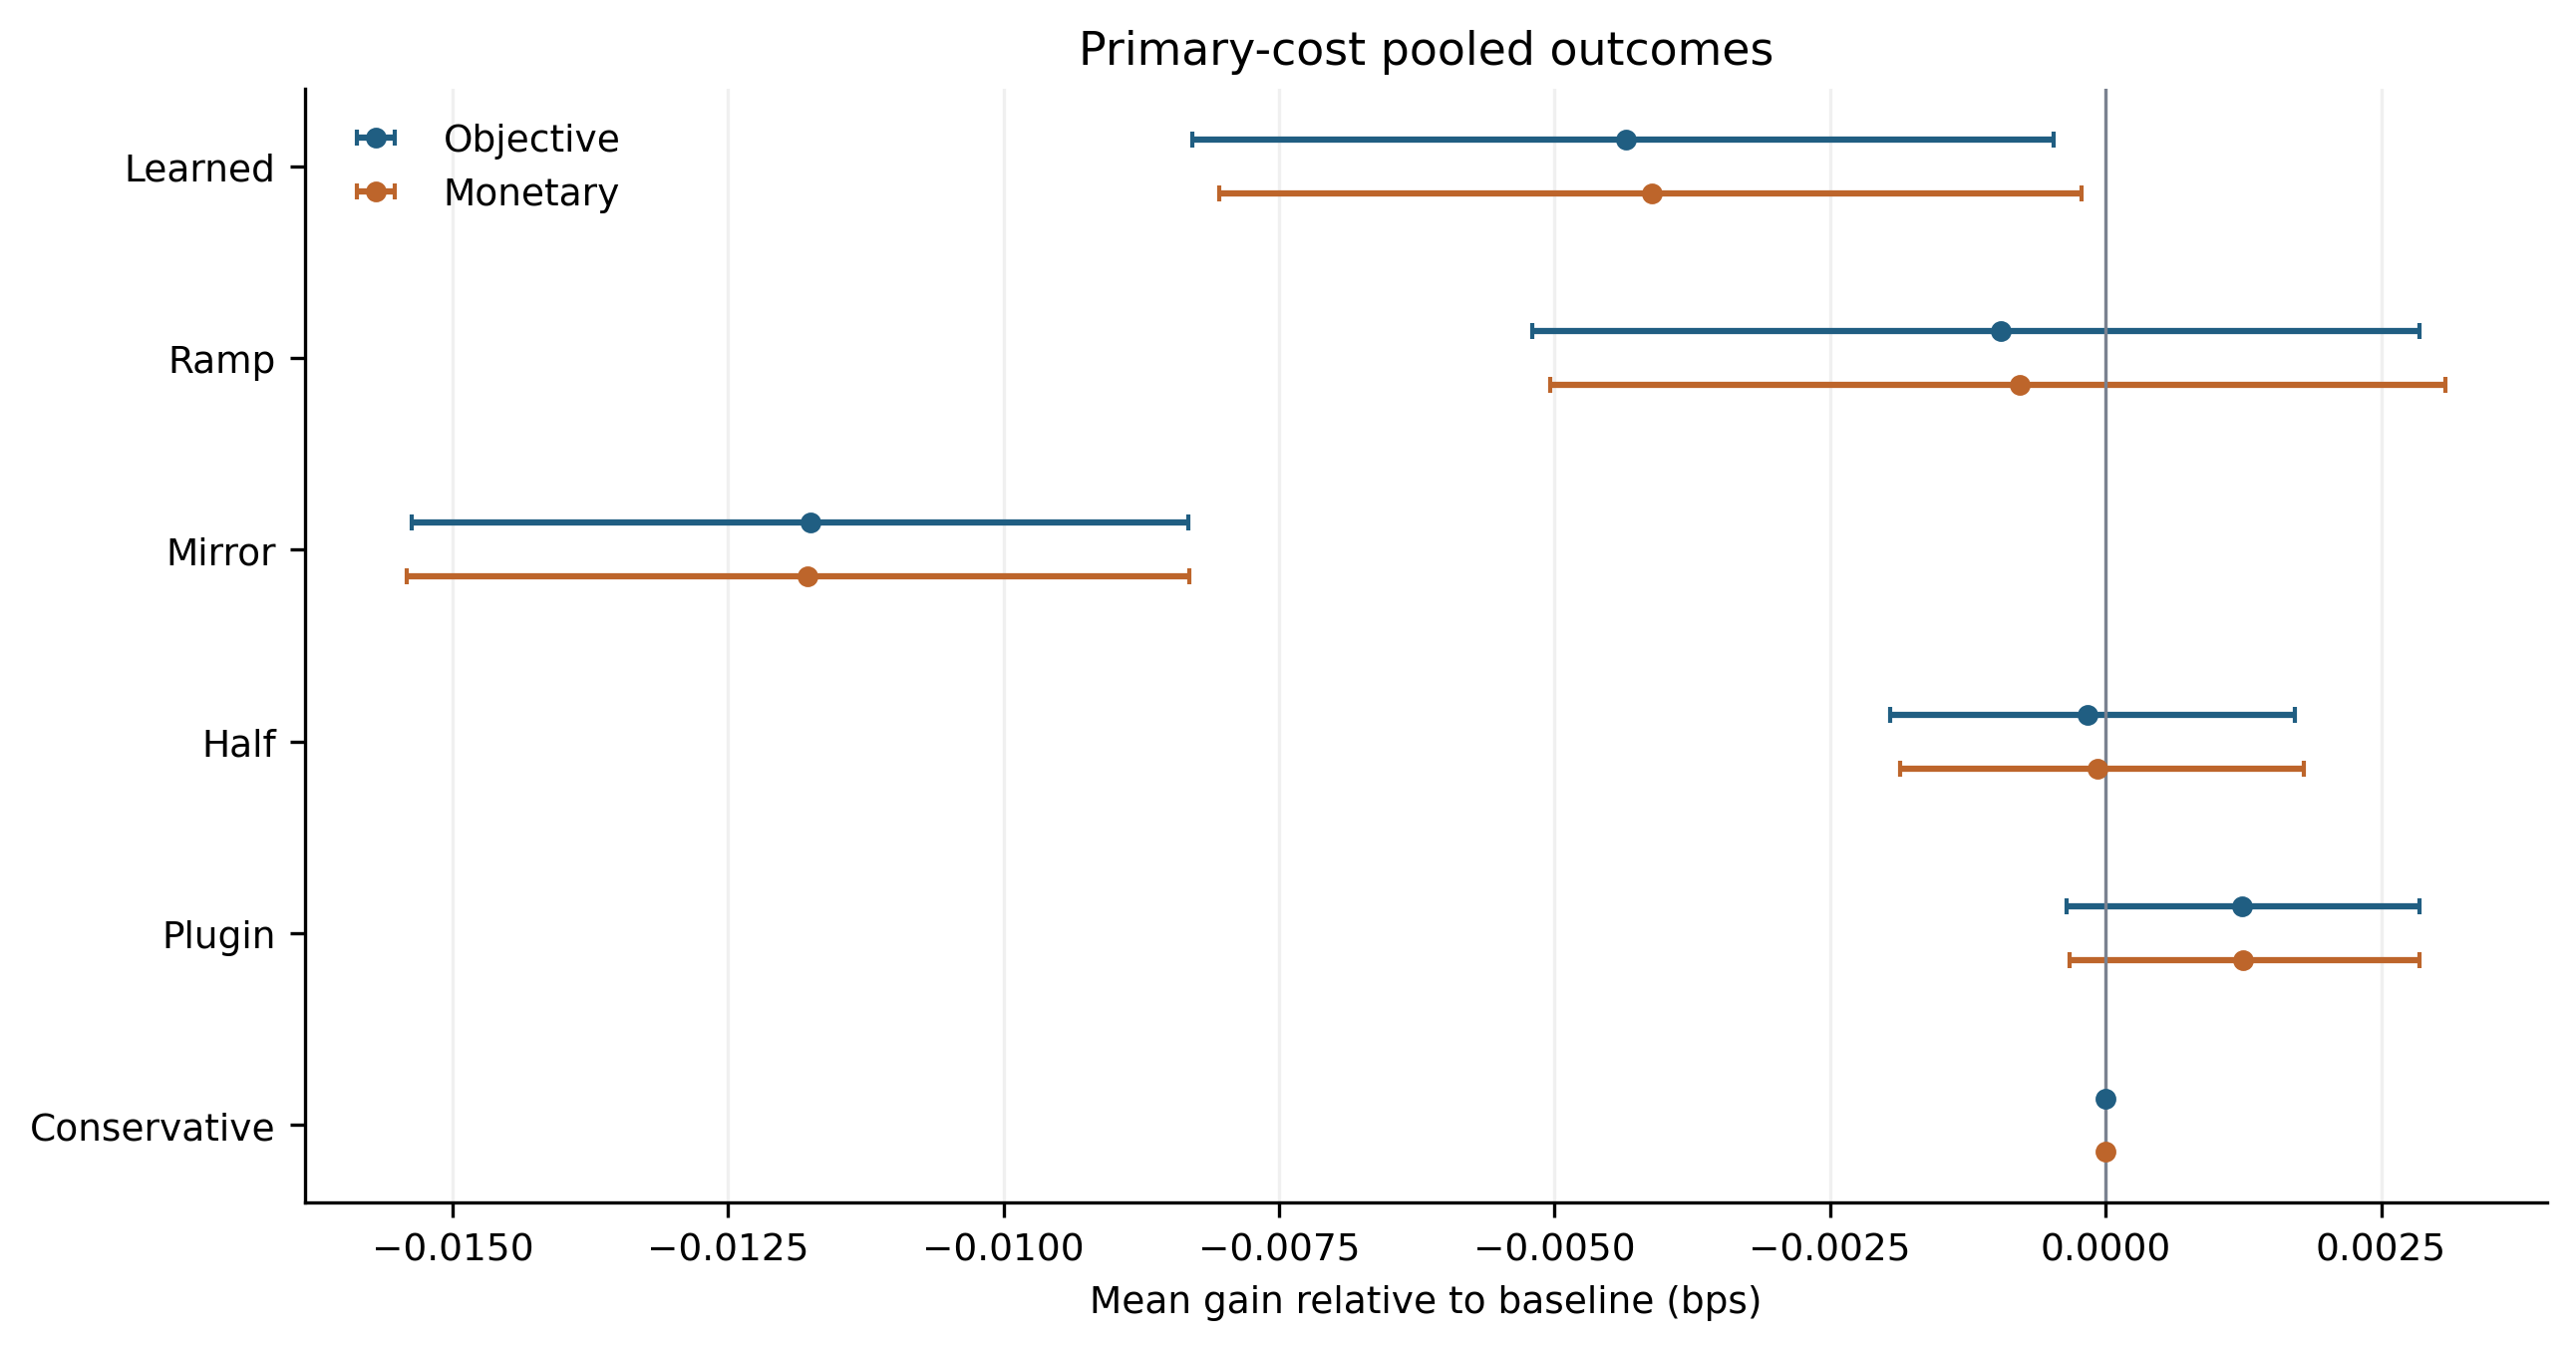
\includegraphics[width=\linewidth]{figures/fig06_objective_monetary.png}
\caption{Primary objective and monetary gains with conditional 95\% day-bootstrap intervals. Monetary scoring removes the inventory preference from the same schedules, while retaining hypothetical impact charges. These are replay outcomes, not observed trading profits.}
\label{fig:monetary}
\end{figure}

Figure~\ref{fig:monetary} separates the two scoring conventions. The inventory term also requires a separate interpretation. At the primary setting, full-exposure monetary gain is $-0.00411$ basis points, compared with objective gain $-0.00436$. Thus the negative conclusion is not generated solely by including a noncash inventory preference. Plug-in monetary gain is $0.00125$ basis points, close to its objective gain. Both monetary measures still contain hypothetical impact charges and minute-open price proxies. Removing the inventory term does not transform them into observed cash savings.

\subsection{Economic interpretation and scope}
The findings support a practical evaluation sequence: distinguish endpoint prediction from temporal price contrasts, examine the schedule induced by those contrasts, and compare its gross timing benefit with the cost of taking that action. This sequence is useful even when the final empirical conclusion is negative. Here endpoint scores cannot distinguish the constructed policies, average learned timing alignment is positive, and full exposure nevertheless reduces the model objective's performance. These are different propositions, each requiring its own evidence.

The present replay cannot establish executable trading gains or a crypto-specific structural mechanism. It lacks parent-order size, quoted spreads, depth, queue position, fill uncertainty and endogenous impact. Bar opens do not verify fills, and an order large enough to change prices would challenge the assumed common realised path. Conversely, an economically richer execution setting might change both relative costs and the appropriate forecast target. The contribution that carries beyond this illustration is the matched-endpoint comparison and benefit--cost accounting, while its quantitative performance conclusions remain conditional on the specified data, schedules and hypothetical costs.

\FloatBarrier
\section{Conclusion}\label{sec:conclusion}
Evaluating a forecast for a fixed-volume execution problem requires attention to the prices available across the execution horizon and to the costs of reallocating the order. A terminal forecast does not identify those temporal contrasts unless additional restrictions connect it to the full price path. The matched-endpoint diagnostic makes that omission explicit while holding terminal-return scores exactly constant. Its economic accounting then asks a separate question: whether the realised benefit of the schedule change pays for the action it induces.

The Bitcoin--Ether illustration shows why these questions should be separated. The learned profile has positive average gross timing alignment under the primary specification, but curvature cost is larger and full exposure produces a negative net objective gain. Historical attenuation changes the balance, yet the reported plug-in interval includes zero and the lower-percentile rule chooses baseline abstention throughout. The sign of the pooled learned gain changes when April is excluded in an ex post descriptive check, showing that the negative mean is concentrated rather than stable across months. Neither policy establishes a generally superior execution procedure. The negative result is informative because the decomposition identifies where the within-model loss arises, rather than attributing it to endpoint accuracy alone.

The evidence supports a practical reporting recommendation: pair the forecast's stated statistical target with its induced schedule, timing payoff, action cost and baseline-relative gain. Those quantities should be distinguished even when a method is not profitable, and their economic scale should be reported alongside uncertainty. Here the primary loss is approximately 0.44 parts per million of reference notional, so statistical detectability cannot establish commercial importance.

A stronger operational assessment would require explicit order sizes, quotes or depth, estimated execution charges, and genuinely prospective evaluation across additional regimes. Competing learned temporal profiles would test whether the diagnostic changes model selection among plausible alternatives. Dependence-sensitive inference and repeated training would address different uncertainties from the present conditional day bootstrap. These extensions could change the empirical performance conclusions; they are not results already obtained. The current study provides a reproducible, deliberately bounded basis for asking those questions, without presenting familiar execution algebra as a new theory or hypothetical gains as attainable trading savings.


\section*{Data and code availability}
{\raggedright The source code, archived market data, checksums, protocols, reported results and editable manuscript are available at \url{https://github.com/JienWeng/crypto-execution-timing}. The data are public Binance spot-market aggregates. The repository identifies the archive sources and distinguishes the reported empirical run from additional descriptive displays. Compiled manuscripts are not included in the repository at this stage.\par}

\section*{Author declarations}
The author has approved the manuscript, authorship and the stated Monash University affiliation. No funding was received for this research. The author declares no competing interests. OpenAI Codex assisted source discovery, mathematical and computational analysis, drafting, figure preparation and internal review. Internal AI reviews are not external journal peer review; responsibility for the manuscript remains with the author. The study uses public aggregate market observations and hypothetical orders, with no human participants, customer-level records or live order placement. No institutional ethics determination or journal submission is asserted.

\begingroup\raggedright
\bibliographystyle{plainnat}
\bibliography{references}
\endgroup
\end{document}
